\documentclass[12pt,a4paper]{article}

% Essential packages
\usepackage[utf8]{inputenc}
\usepackage[T1]{fontenc}
\usepackage{graphicx}
\usepackage{amsmath,amssymb}
\usepackage{algorithm}
\usepackage{algpseudocode}
\usepackage{booktabs}
\usepackage{hyperref}
\usepackage[margin=1in]{geometry}
\usepackage{float}
\usepackage{caption}
\usepackage{subcaption}
\usepackage{placeins}

% New beautification packages
\usepackage{tocloft}           % Better ToC formatting
\usepackage{titlesec}          % Custom section formatting
\usepackage{enumitem}          % Better list formatting
\usepackage{microtype}         % Micro-typography improvements
\usepackage{setspace}          % Line spacing control
\usepackage{xcolor}            % Already included
\usepackage{colortbl}          % Color in tables
\usepackage{listings}          % Already included
\usepackage{fancyhdr}          % Already included
\usepackage{url}               % Better URL formatting

\pagestyle{fancy}
\fancyhf{}
\rhead{Histogram Equalization and Matching}
\lhead{Digital Image Processing}
\rfoot{Page \thepage}

\setlength{\parindent}{0pt}    % No paragraph indentation
\setlength{\parskip}{8pt}      % Space between paragraphs


% Colors for document
\definecolor{sectcolor}{RGB}{70,30,80}
\definecolor{linkcolor}{RGB}{0,120,215} 
\definecolor{tableheader}{RGB}{240,240,255}

% Section formatting
\titleformat{\section}
  {\normalfont\Large\bfseries\color{sectcolor}}{\thesection}{1em}{}
\titleformat{\subsection}
  {\normalfont\large\bfseries\color{sectcolor}}{\thesubsection}{1em}{}

% Hyperref setup
\hypersetup{
    colorlinks=true,
    linkcolor=linkcolor,
    citecolor=citecolor,
    urlcolor=linkcolor,
    pdfborder={0 0 0},
}

% List formatting
\setlist{itemsep=4pt, topsep=6pt}



% Document information
\title{\Large \textbf{Histogram Equalization and Matching:\\A Comparative Analysis of Different Approaches}}
\author{Fraidakis Ioannis\\
\small Department of Electrical and Computer Engineering\\
\small Aristotle University of Thessaloniki}
\date{April 2025}

\begin{document}

\maketitle

\begin{abstract}
This report presents an implementation and analysis of various histogram modification techniques for digital images. Three different algorithms for histogram equalization and matching are compared: greedy, non-greedy, and post-disturbance approaches. We study how these algorithms transform image intensity distributions and analyze their effectiveness through both visual assessment and quantitative metrics. Experimental results demonstrate the strengths and limitations of each approach when applied to real-world images, with particular attention to their impact on image contrast enhancement and intensity distribution matching.
\end{abstract}

\section{Introduction}

In digital image processing, the quality and usability of images often depend not on their absolute pixel values, but on how these values are distributed across the available intensity range. Histogram-based techniques stand as powerful tools for manipulating this distribution, enabling significant enhancements without altering the fundamental content of an image. This report focuses on two critical histogram operations: histogram equalization (Section~\ref{subsec:histogram_equalization}) and histogram matching (Section~\ref{subsec:histogram_matching}).

This study specifically addresses the following objectives:

\begin{itemize}
    \item Implement and compare three fundamentally different algorithmic approaches to histogram manipulation: greedy, non-greedy, and post-disturbance methods
    \item Evaluate the visual impact of each method on real-world grayscale images
    \item Quantitatively assess algorithm performance through multiple similarity metrics measuring how accurately each achieves target histograms
    \item Investigate the effectiveness of post-processing techniques like dynamic range stretching as a remedy for underutilized intensity ranges
\end{itemize}


\section{Theoretical Background}

\subsection{Image Histograms}

The histogram of a digital grayscale image represents the statistical distribution of pixel intensities across the available dynamic range. Formally, for an image with intensity values in the range $[0,1]$, the histogram $h(i)$ counts the number of pixels with intensity value $i$. The normalized histogram $p(i) = h(i)/n$ (where $n$ is the total number of pixels) provides the probability density function of intensity levels within the image.

This statistical representation offers valuable insights into an image's tonal characteristics:
\begin{itemize}
    \item \textbf{Dynamic range utilization:} The width of the histogram indicates how effectively the image uses the available intensity range
    \item \textbf{Brightness:} The central tendency of the histogram reflects overall image brightness—histograms skewed toward higher values indicate brighter images, while those concentrated in lower ranges suggest darker content
    \item \textbf{Contrast:} The spread of the histogram corresponds to image contrast—tightly clustered histograms indicate low contrast, while broadly distributed histograms suggest higher contrast
    \item \textbf{Exposure quality:} Histograms pressed against either extreme (0 or 1) may indicate under or overexposure with potentially lost detail
\end{itemize}



\subsection{Histogram Equalization}
\label{subsec:histogram_equalization}

Histogram equalization is a technique that enhances image contrast by redistributing intensity values. The goal is to transform an image such that its histogram becomes approximately uniform across the available intensity range.

This transformation redistributes pixel intensities such that areas of high local density in the original histogram are stretched over a wider range, while areas of low density are compressed. The process is particularly effective for images with poor contrast due to limited dynamic range utilization, revealing details that would otherwise remain hidden.

\subsection{Histogram Matching}
\label{subsec:histogram_matching}

Histogram matching (also known as histogram specification) is a process that transforms the intensity distribution of an image to resemble a specified reference histogram. Unlike equalization, which aims for uniformity, matching allows an image to adopt the tonal characteristics of another image.

This technique is valuable when e.g. standardizing images taken under different lighting conditions or when aiming to achieve a specific aesthetic quality. By transferring the intensity distribution from a well-balanced reference image to a poorly exposed input image, details can be enhanced while maintaining a natural appearance.




\section{Implementation Framework}

\subsection{Code Architecture}

The codebase is structured around the principle of modular design:

\begin{itemize}
    \item \textbf{Histogram utilities} (\texttt{hist\_utils.py}): Provides core functions for computing image histograms and applying transformation mappings.
    
    \item \textbf{Modification algorithms} (\texttt{hist\_modif.py}): Implements the three histogram modification approaches (greedy, non-greedy, post-disturbance) with clean, consistent interfaces for both equalization and matching operations.
    
    \item \textbf{Evaluation metrics} (\texttt{metrics.py}): Defines quantitative measures for assessing histogram modifications, including various similarity metrics to evaluate how well the transformed histogram matches the target.

    \item \textbf{Visualization utilities} (\texttt{image\_utils.py}): Centralizes image handling, visualization, and results presentation functionality, including styled figure creation, image display, and performance metrics reporting.

    \item \textbf{Demonstration script} (\texttt{demo.py}): Orchestrates the experiments, processes the workflow, and generates comparative visualizations.
\end{itemize}


\subsection{Technical Dependencies}

The implementation leverages standard scientific computing libraries to ensure reliability, performance, and reproducibility:

\begin{itemize}
    \item \textbf{NumPy:} Provides the foundation for efficient numerical operations and array manipulations, serving as the core data structure for image representation and histogram calculations. The implementation uses NumPy's advanced indexing, broadcasting capabilities, and vectorized operations to optimize performance.
    
    \item \textbf{Pillow (PIL):} Handles image file I/O operations, format conversion, and image manipulations. This library ensures compatibility with various image formats and provides essential preprocessing capabilities for converting color images to grayscale.
    
    \item \textbf{Matplotlib:} Enables comprehensive visualization of results through its extensive plotting capabilities. The implementation uses Matplotlib for generating comparative visualizations of original and processed images alongside their corresponding histograms, with customized styling for clear presentation.
        \item \textbf{SciPy:} Provides specialized scientific functions, particularly the Wasserstein distance (Earth Mover's Distance) implementation used for histogram comparison metrics.
    
    \item \textbf{Pandas:} Facilitates data organization, display, and export of quantitative results, allowing for clear tabular presentation of evaluation metrics and save to CSV files.

\end{itemize}


\subsection{Implementation Workflow}

The processing pipeline follows a consistent sequence of operations:

\begin{enumerate}
    \item \textbf{Image acquisition and preprocessing:} Loading images from disk, converting to grayscale if needed, and normalizing pixel values to the [0,1] range.
    
    \item \textbf{Histogram analysis:} Calculating the initial histogram of the input image and, for matching operations, the reference histogram.
    
    \item \textbf{Intensity mapping:} Applying the selected algorithm (greedy, non-greedy, or post-disturbance) to generate a mapping between input and target intensity values.
    
    \item \textbf{Image transformation:} Applying the derived mapping to create the output image with the modified histogram.
    
    \item \textbf{Evaluation and visualization:} Calculating similarity metrics between achieved and target histograms, and generating comparative visualizations.
\end{enumerate}



\section{Proposed Histogram Modification Algorithms}

This study implements and compares three distinct algorithms for histogram modification: greedy, non-greedy, and post-disturbance approaches. Each algorithm represents a different strategy for mapping input intensity values to output intensity values, with varying trade-offs between computational simplicity and histogram accuracy.

\subsection{Greedy Algorithm}

The greedy algorithm implements a straightforward, sequential approach to histogram modification by prioritizing complete bin filling. Operating on sorted intensity values, this method assigns input pixels to output bins in order until each target bin reaches or exceeds its required capacity. This computationally efficient approach is characterized by its deterministic behavior and simplicity. The pseudocode below outlines this process:


\begin{algorithm}[H]
    \caption{Greedy Histogram Matching}
    \begin{algorithmic}[1]
        \State Sort input intensities $\{r_i\}$ and output intensities $\{z_j\}$
        \State Set current input index $i \gets 0$
        \For{each output intensity $z_j$ in sorted order}
            \State Get target pixel count $target_j$ for $z_j$
            \State Initialize accumulated pixels $a \gets 0$
            \While{$i < \text{length}(\{r_i\})$ \textbf{and} $a < target_j$}
            \State Get current input intensity $r_i$ and its pixel count $count_i$       \State Map $r_i \mapsto z_j$ (add to histogram mapping)
                \State $a \gets a + count_i$
                \State $i \gets i + 1$
            \EndWhile
        \EndFor
    \end{algorithmic}
\end{algorithm}

A key limitation of this approach is its handling of large input intensity groups. When a single input intensity has many pixels, the algorithm assigns all these pixels to just one output bin, potentially causing that bin to be significantly overfilled. As some bins become overfilled early in the process, there may not be enough pixels remaining to fill the entire target intensity range. This can result in higher-intensity output bins (toward the right end of the histogram) remaining empty, preventing full utilization of the available dynamic range and limiting the contrast enhancement in brighter regions of the transformed image. 


\subsection{Non-Greedy Algorithm}

The non-greedy algorithm partially addresses the limitations of the greedy approach by incorporating a decision rule for bin assignment. An input intensity group is assigned to the current output bin only if:

\begin{enumerate}
    \item It is the first group being assigned to that bin, or
    \item At least half of its pixels would fit in the remaining bin capacity
\end{enumerate}

When significant overflow would occur (i.e., less than half of the pixels from the current input intensity would fit in the remaining bin capacity), the algorithm advances to the next output bin. This approach reduces extreme bin overfilling but doesn't solve the fundamental issue—pixels from a single input intensity still map to exactly one output bin, a limitation only the post-disturbance approach overcomes.

The non-greedy algorithm maintains computational efficiency comparable to the greedy method while yielding more visually coherent results. By considering bin capacity before making assignments, it produces a mapping function with fewer sharp discontinuities, resulting in smoother intensity transitions in the output image.

\subsection{Post-Disturbance Algorithm}

The post-disturbance algorithm takes a fundamentally different approach by addressing the discrete nature of digital image intensities. Rather than directly mapping the original intensity values, this method first transforms the input image into a more continuous distribution through controlled noise addition.

The algorithm works through the following key steps:

\begin{algorithm}[H]
    \caption{Post-Disturbance Histogram Matching}
    \begin{algorithmic}[1]
        \State Get unique intensity values $\{r_i\}$ from input histogram
        \State Sort unique values
        \State Calculate step size $d = r_1 - r_0$ (difference between first two values)
        \State Generate random noise matrix $noise \sim Uniform(-d/2, d/2)$ 
        \State Add noise to input image: $noisy\_image = img\_array + noise$
        \State Clip values to valid range: $noisy\_image = clip(noisy\_image, 0, 1)$
        \State Apply greedy histogram matching to $noisy\_image$ using reference histogram
        \State \Return resulting matched image
    \end{algorithmic}
\end{algorithm}

The addition of uniform random noise ($n \in [-d/2, d/2]$, where $d$ is the typical intensity step) effectively breaks up clusters of identical pixel values into slightly different intensities. The noise magnitude is carefully controlled to be proportional to $d$, ensuring that the introduced disturbance preserves the original intensity ordering. This transforms the discrete input histogram into a continuous distribution, enabling fine-grained mapping between input and target histograms. 

This method is particularly effective for images with large uniform areas or limited unique intensity values, where traditional histogram modification methods can produce visible posterization effects.

\subsection{Supporting Functions}

The implementation relies on several core utility functions that provide essential services to the main histogram modification algorithms:

\subsubsection*{Histogram Calculation (\texttt{hist\_utils.py/calculate\_hist\_of\_img})}
This function performs the task of computing the intensity distribution of an image:

\begin{itemize}
    \item It identifies all unique intensity values present in the image array and counts their occurrences
    \item The function supports both raw count output (for internal algorithm processing) and normalized histograms (for probability distribution analysis and visualization)
\end{itemize}

\subsubsection*{Histogram Equalization (\texttt{hist\_modif.py/perform\_hist\_eq})}
This wrapper function implements the standard histogram equalization process:

\begin{itemize}
    \item Constructs a target uniform histogram with discrete levels $s_k = \frac{k}{L_g-1}$ for $k = 0,1,...,L_g-1$, where $L_g=256$ represents standard 8-bit precision
    \item Assigns equal probability mass $p_T(s_k) = \frac{1}{L_g}$ to each output level, ensuring uniform distribution
\end{itemize}


\subsubsection*{Histogram Matching (\texttt{hist\_modif.py/perform\_hist\_matching})}
This function orchestrates the process of matching one image's histogram to another:

\begin{itemize}
    \item Extracts the normalized histogram from the reference image to serve as the target probability distribution
    \item The core modification algorithm (specified by mode) is then applied to map input intensities to the reference distribution
\end{itemize}



\newpage


\section{Experimental Setup}

\subsection{Test Images}

Our experiments used two test images with different characteristics:
\begin{itemize}
    \item \textbf{Input Image}: The source image to be modified (a cat resting on a couch), originally in color but converted to grayscale for our experiments.
    \item \textbf{Reference Image}: The target image whose histogram is used as reference for matching (a person in a dimly lit room), characterized by predominantly dark tones.
\end{itemize}
\begin{figure}[H]
    \centering
    \begin{subfigure}{\textwidth}
        \centering
        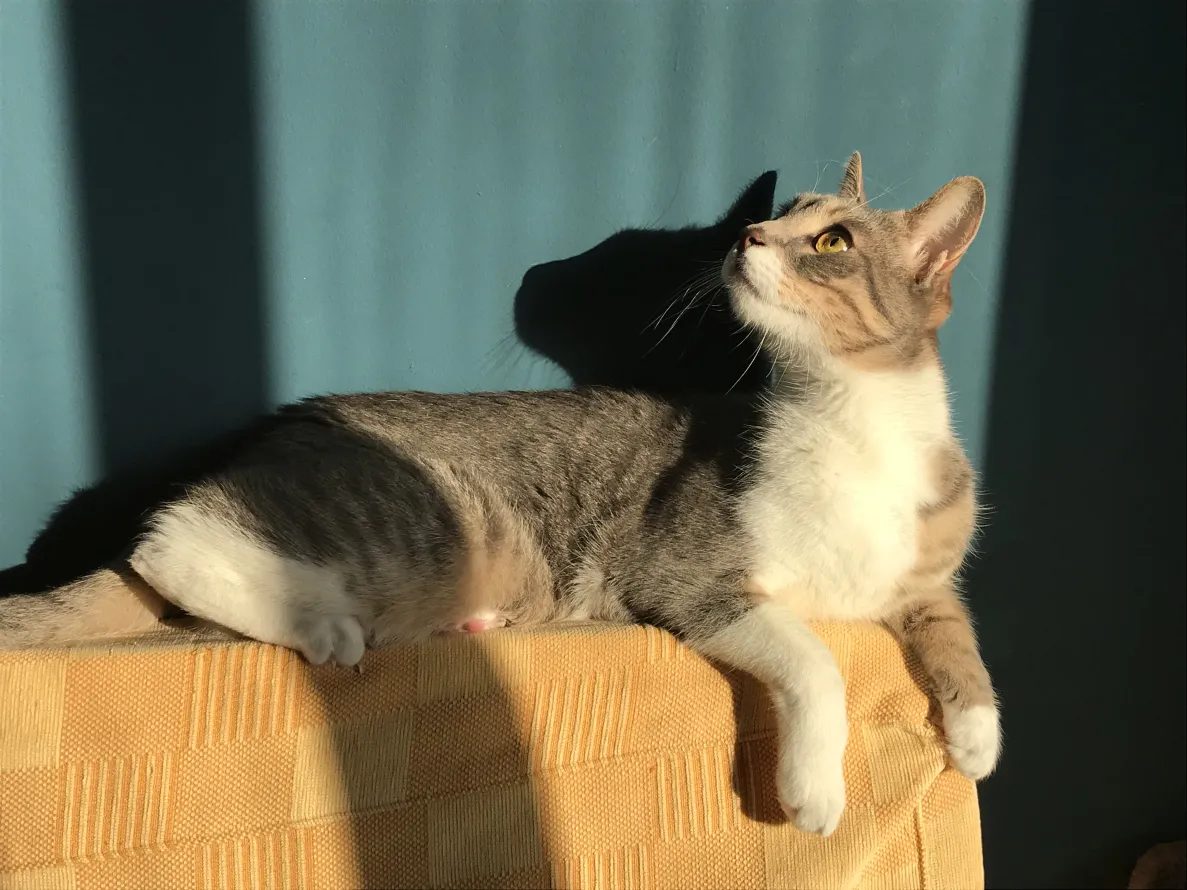
\includegraphics[width=0.6\textwidth]{hw1_images/input_img.jpg}
        \caption{Input Image}
    \end{subfigure}
    
    \vspace{0.8cm}
    
    \begin{subfigure}{\textwidth}
        \centering
        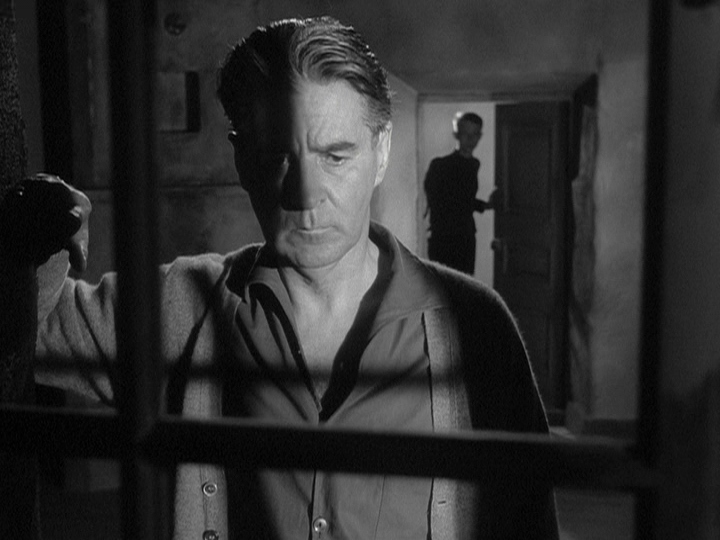
\includegraphics[width=0.6\textwidth]{hw1_images/ref_img.jpg}
        \caption{Reference Image}
    \end{subfigure}
    \caption{Test images used in the experiments.}
    \label{fig:test_images}
\end{figure}

\subsection{Evaluation Metrics}

To objectively quantify algorithm performance, we employed four complementary histogram similarity metrics. Each metric captures different aspects of the relationship between achieved and target histograms:

\begin{itemize}
    \item \textbf{Mean Squared Error (MSE):} Measures the average squared difference between the achieved histogram $h_1$ and the target histogram $h_2$:
    \begin{equation}
        \text{MSE} = \frac{1}{n}\sum_{i=1}^{n}(h_1(i) - h_2(i))^2
    \end{equation}
    where $n$ is the number of intensity levels. MSE is sensitive to differences at all intensity levels and penalizes larger deviations more heavily due to the squaring operation. Lower values indicate better performance, with a perfect match yielding MSE = 0.
    \item \textbf{Bhattacharyya Distance:} Quantifies the similarity between two probability distributions and is particularly useful for comparing normalized histograms:
    \begin{equation}
        D_B(h_1, h_2) = -\ln\left(\sum_{i=1}^{n}\sqrt{h_1(i) \cdot h_2(i)}\right)
    \end{equation}
    This metric is bounded between 0 (identical distributions) and $\infty$ (completely different distributions). The Bhattacharyya distance is less sensitive to outliers than MSE and provides a good measure of overall distribution similarity.
    
    \item \textbf{Histogram Intersection:} Calculates the overlap between two normalized histograms:
    \begin{equation}
        I(h_1, h_2) = \sum_{i=1}^{n} \min(h_1(i), h_2(i))
    \end{equation}
    This metric ranges from 0 (no overlap) to 1 (perfect match). It directly measures how much of one distribution is shared with the other, making it intuitive to interpret. Higher values indicate better matching.
    
    \item \textbf{Earth Mover's Distance (EMD):} Measures the minimum cost required to transform one histogram into another, conceptualized as the work needed to move "probability mass" between bins:
    \begin{equation}
        \text{EMD}(h_1, h_2) = \inf_{\gamma \in \Gamma(h_1, h_2)} \int d(x, y) d\gamma(x, y)
    \end{equation}
    where $\Gamma(h_1, h_2)$ is the set of all possible ways to transfer mass from $h_1$ to $h_2$, and $d(x, y)$ is the ground distance between bins. EMD is particularly valuable for histogram comparison because it accounts for the perceptual difference between intensity levels, not just bin-by-bin differences. Lower values indicate better performance.
\end{itemize}


\section{Experimental Results and Analysis}

This section presents both qualitative and quantitative evaluation of the implemented histogram modification algorithms. We analyze performance in two distinct tasks: histogram equalization (Section~\ref{subsec:histogram_equalization}) and histogram matching (Section~\ref{subsec:histogram_matching}).
\subsection{Histogram Equalization}

\subsubsection{Visual Results}

Figure~\ref{fig:eq_comp} presents a comprehensive comparison of the three histogram equalization algorithms. The left column shows the original input image and the transformed results from each method, while the right column displays the corresponding intensity distributions alongside the target uniform histogram (dashed yellow line).

\begin{figure}[H]
    \centering
    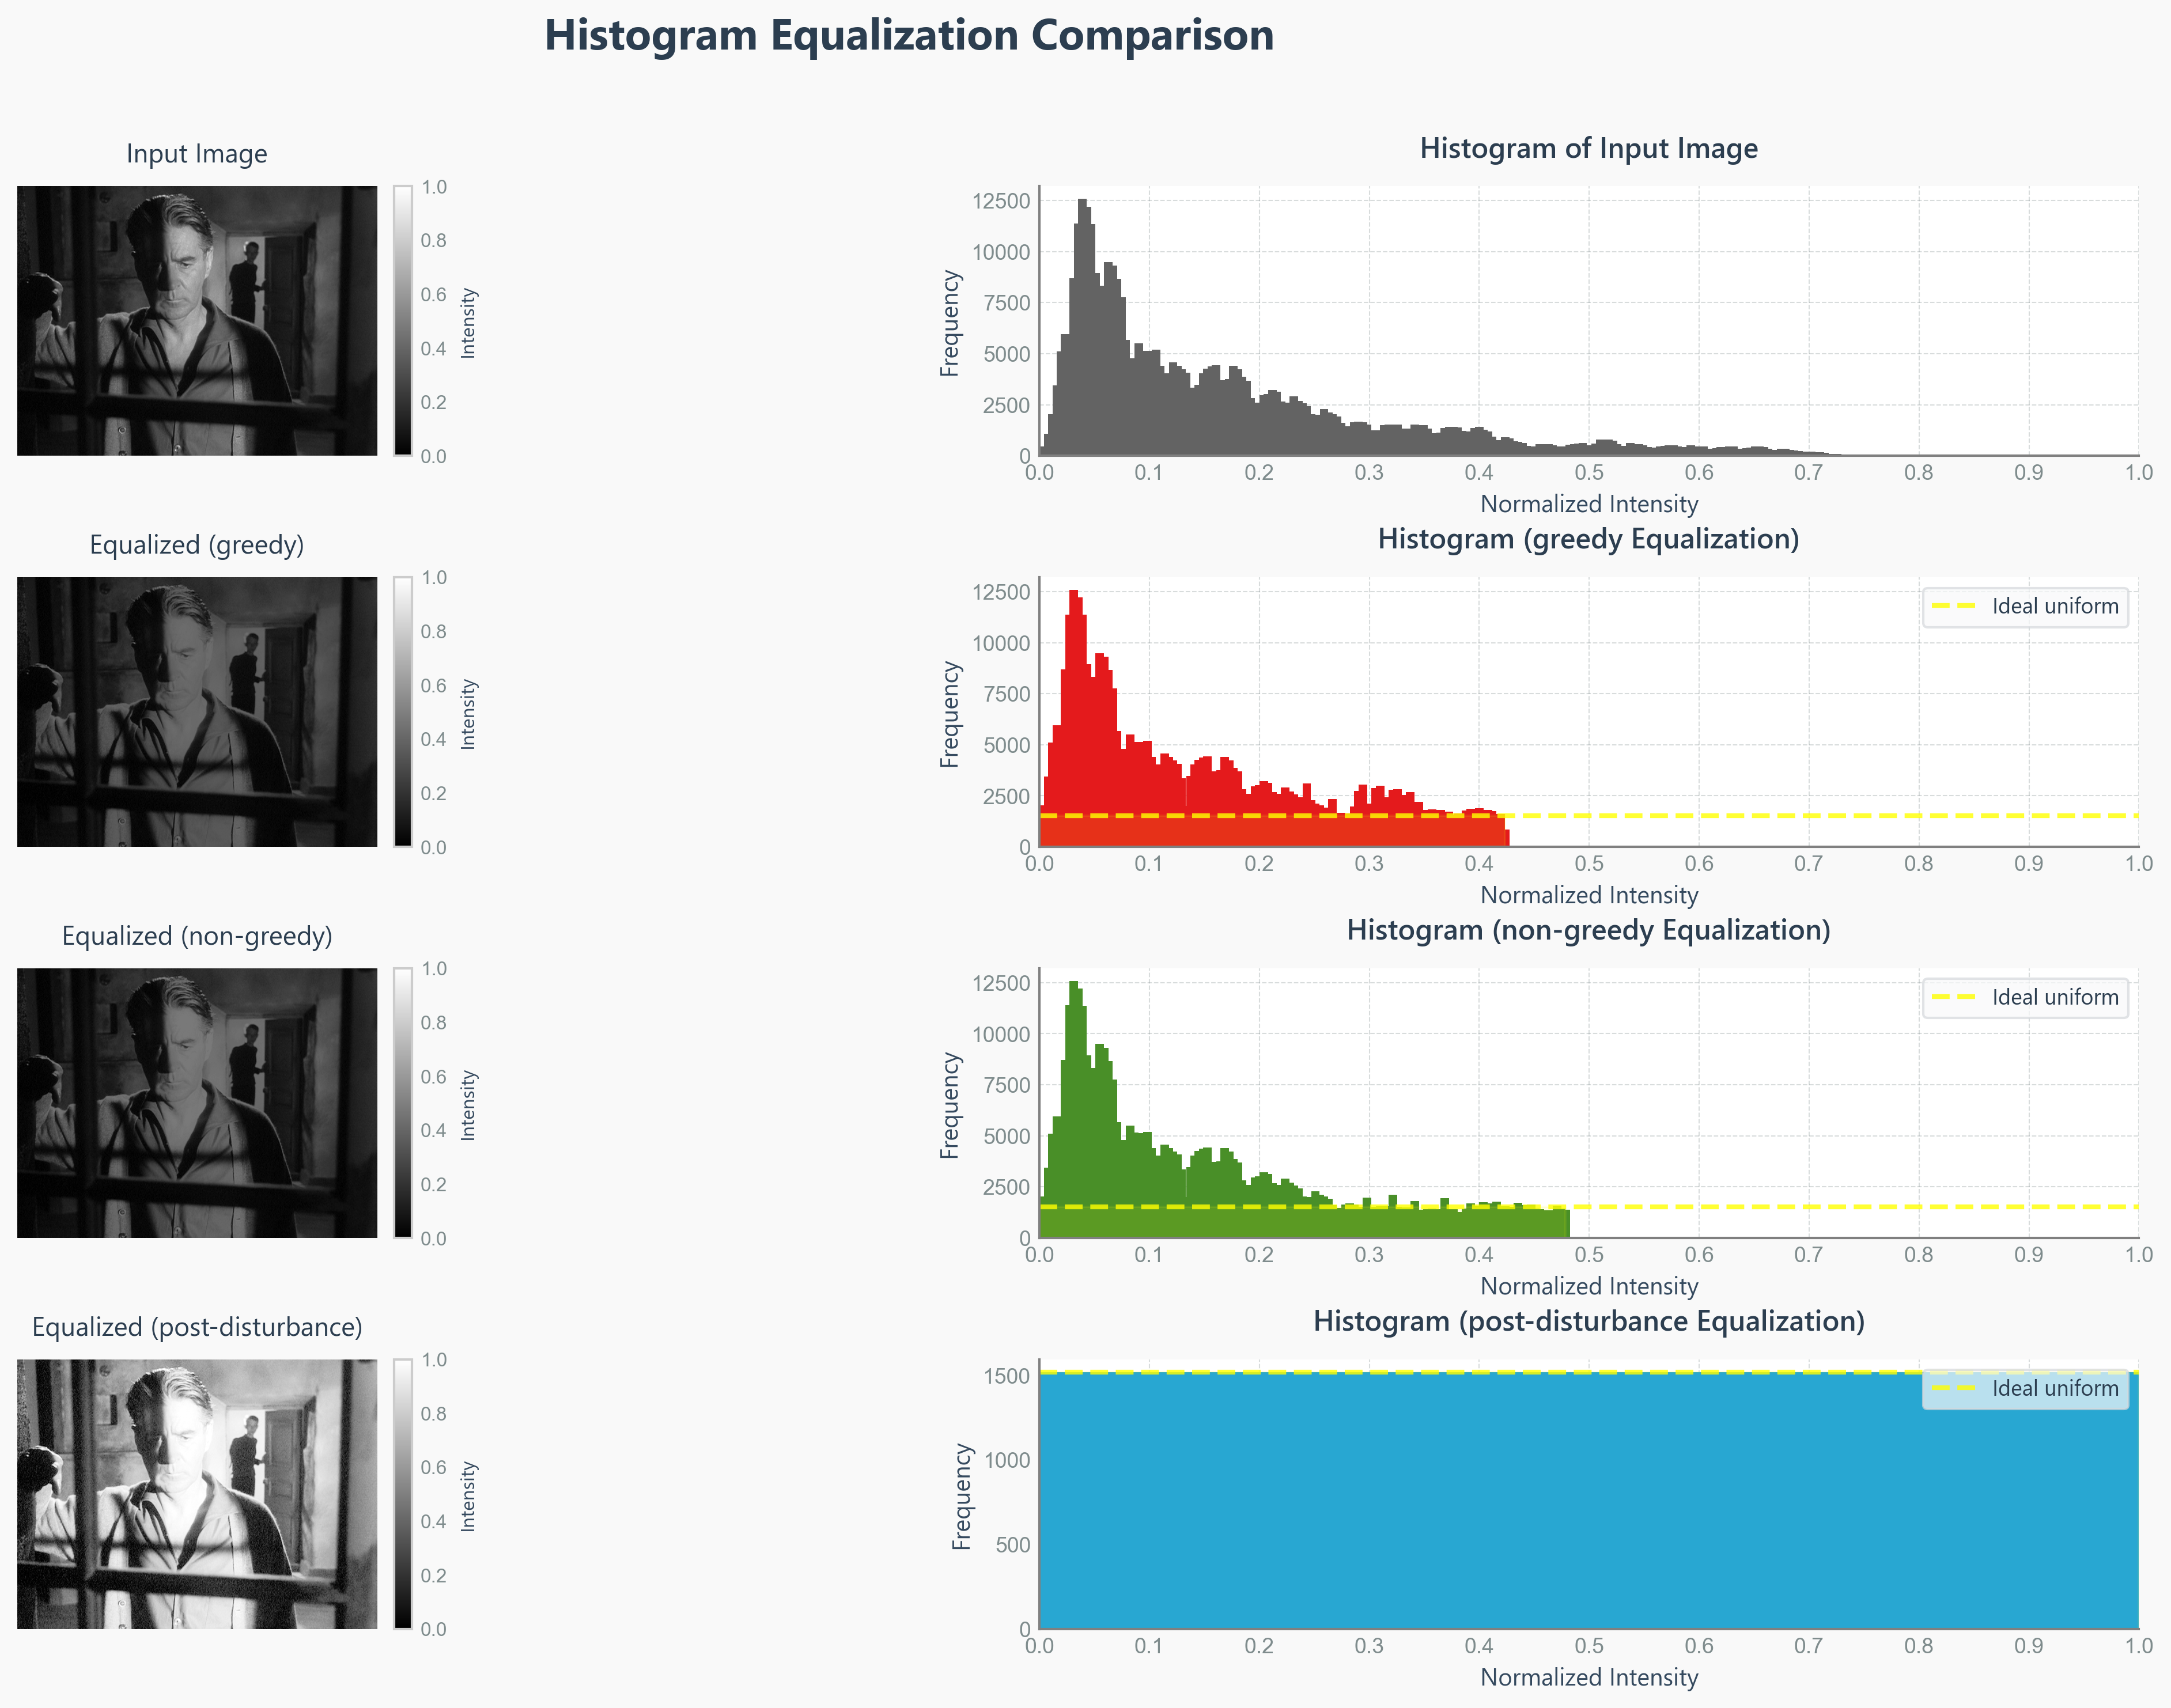
\includegraphics[width=\textwidth]{results/images/histogram_equalization_comparison.png}
    \caption{Comparison of Histogram Equalization Modes.}
    \label{fig:eq_comp}
\end{figure}


\subsubsection{Histogram Analysis}\label{HistogramAnalysis}

Examining the histograms reveals characteristic differences in how each algorithm redistributes pixel intensities:

\begin{itemize}
    \item \textbf{Input Image:} The original image exhibits a bimodal histogram with a significant peak in the darker region (around 0.1 intensity) and a secondary peak in the mid-tones (around 0.45 intensity). This distribution indicates limited contrast and overall poor utilization of the entire dynamic range, particularly in the brighter regions (0.6-1.0) where very few pixels are present. This concentration of values in specific intensity ranges rather than across the full spectrum limits the image's visual impact.

    \item \textbf{Greedy Equalization:} The resulting histogram maintains peaks at similar positions to the original with better distribution in the mid-range (0.1-0.5). However, it shows significant clustering in the lower intensity range (0.0--0.1) with several pronounced peaks throughout. Despite equalization, the output histogram still exhibits poor utilization of higher intensity values (above 0.6), only extending to approximately 0.58 on the intensity scale and failing to utilize the full [0,1] range. This limitation occurs because large input intensity groups are mapped entirely to single output levels, creating oversaturated bins and leaving others empty. See Appendix~\ref{appendix:stretching} for a post-processing stretching technique that addresses this limitation.


    \item \textbf{Non-Greedy Equalization:} This histogram demonstrates a similar peak structure to the greedy approach but with a slightly better spread across the intensity range. The algorithm pushes more pixels toward higher intensity values (approximately 0.7), creating a more balanced distribution that extends further than the greedy method. The strategic bin assignment rule effectively mitigates some of the clustering issues.    

    \item \textbf{Post-Disturbance Equalization:} This method produces a remarkably uniform histogram that spans the entire [0,1] range and closely matches the ideal uniform distribution. The controlled noise addition successfully transforms the discrete input histogram into a continuous distribution, allowing for precise intensity mapping and complete elimination of the clustering artifacts seen in the other methods.
\end{itemize}

\subsubsection{Visual Quality Assessment}

Figure~\ref{fig:eq_images} highlights the differences between the three equalized images:

\begin{figure}[H]
    \centering
    \begin{subfigure}{0.32\textwidth}
        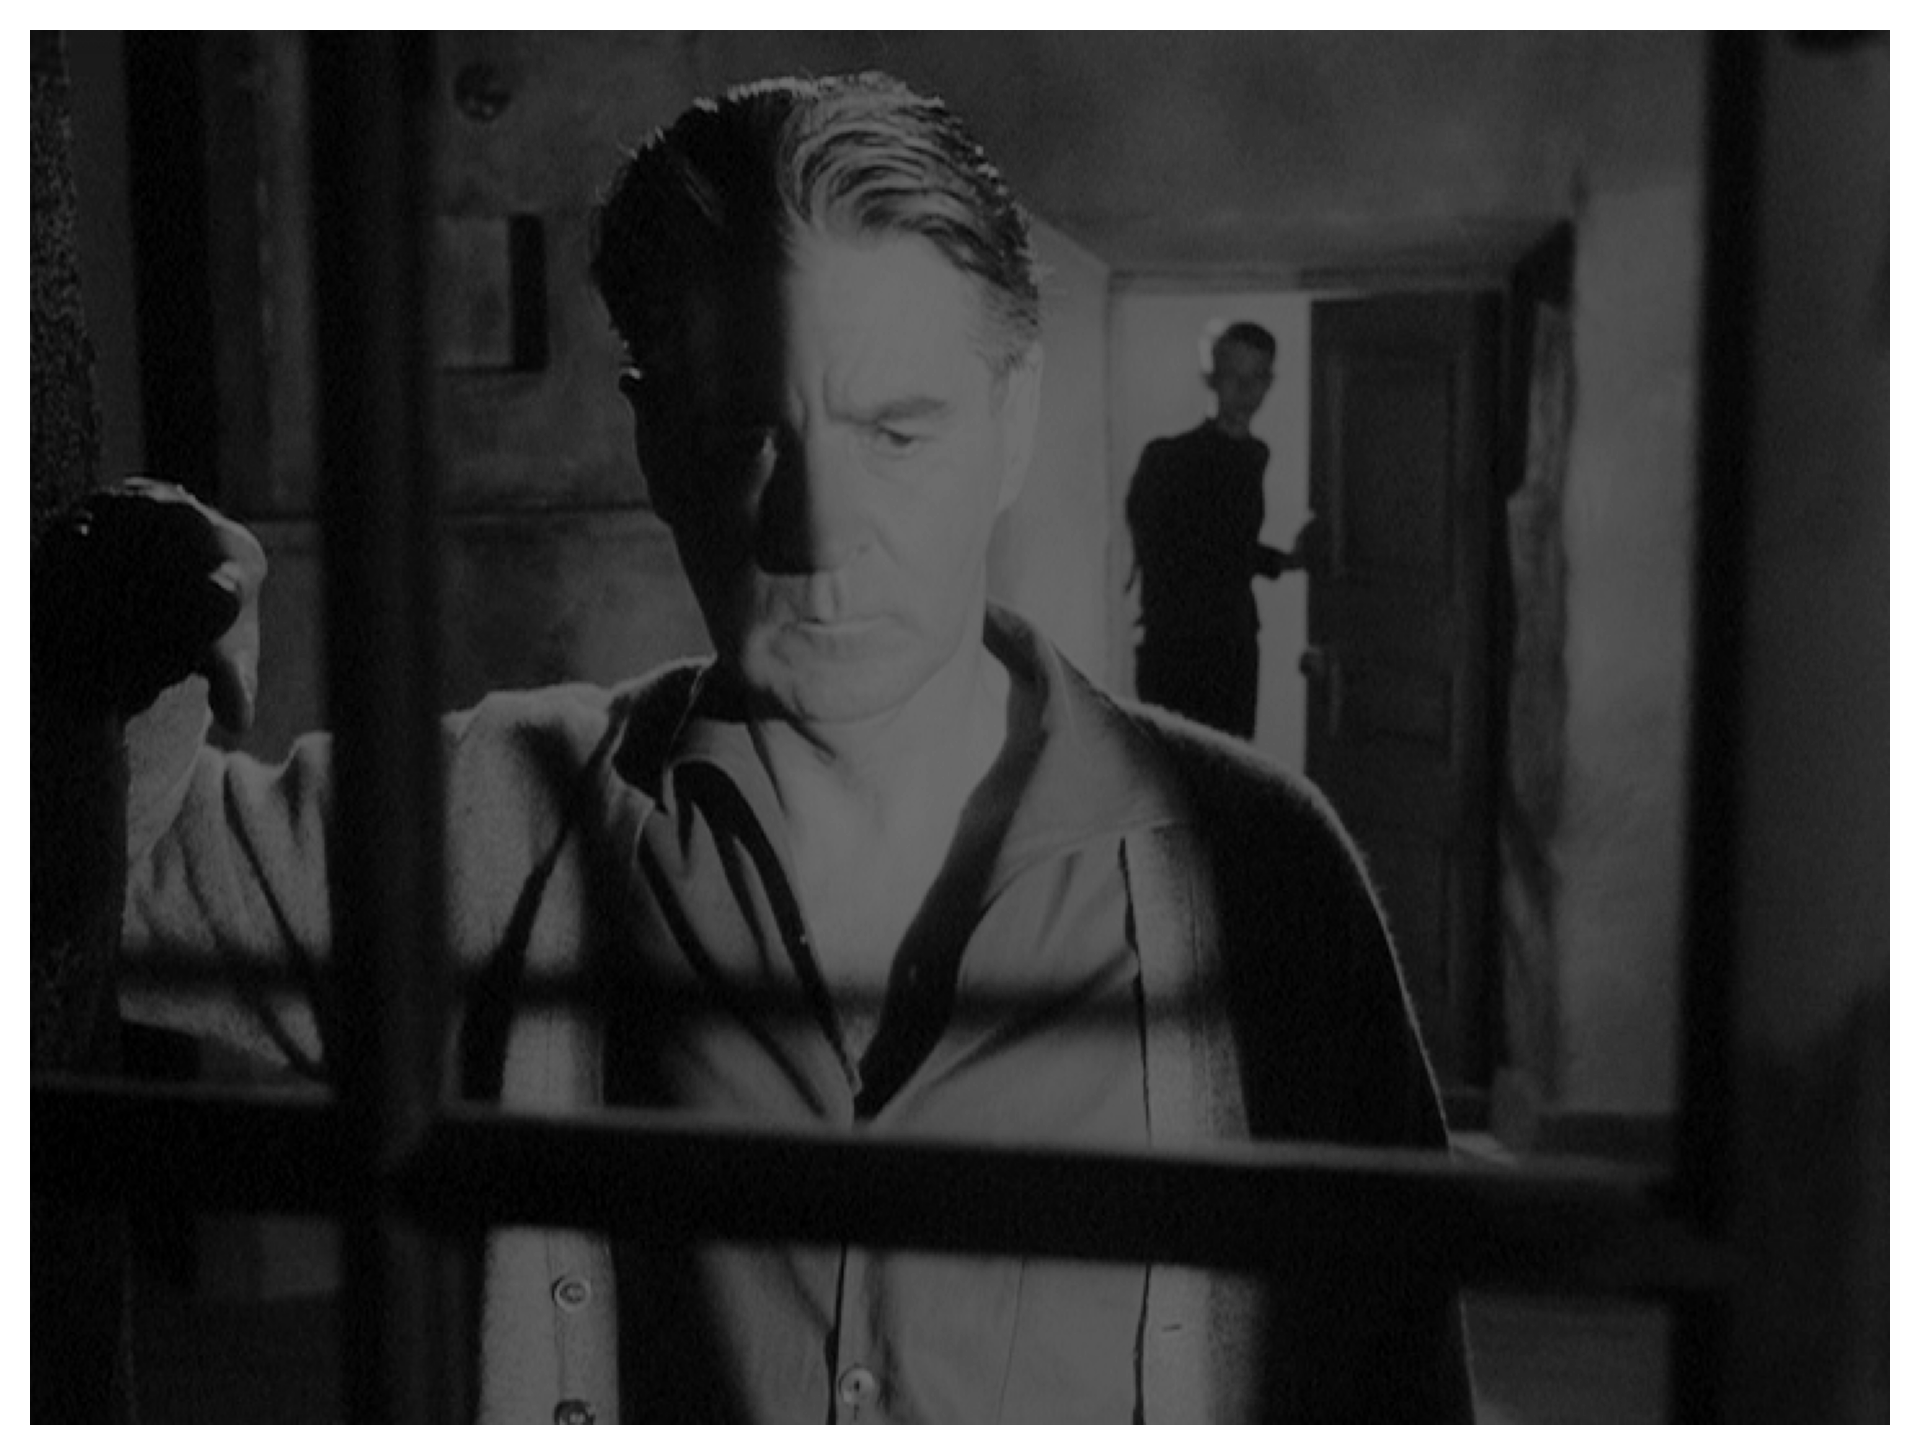
\includegraphics[width=\textwidth]{results/images/equalized_greedy.png}
        \caption{Greedy Equalization}
    \end{subfigure}
    \hfill
    \begin{subfigure}{0.32\textwidth}
        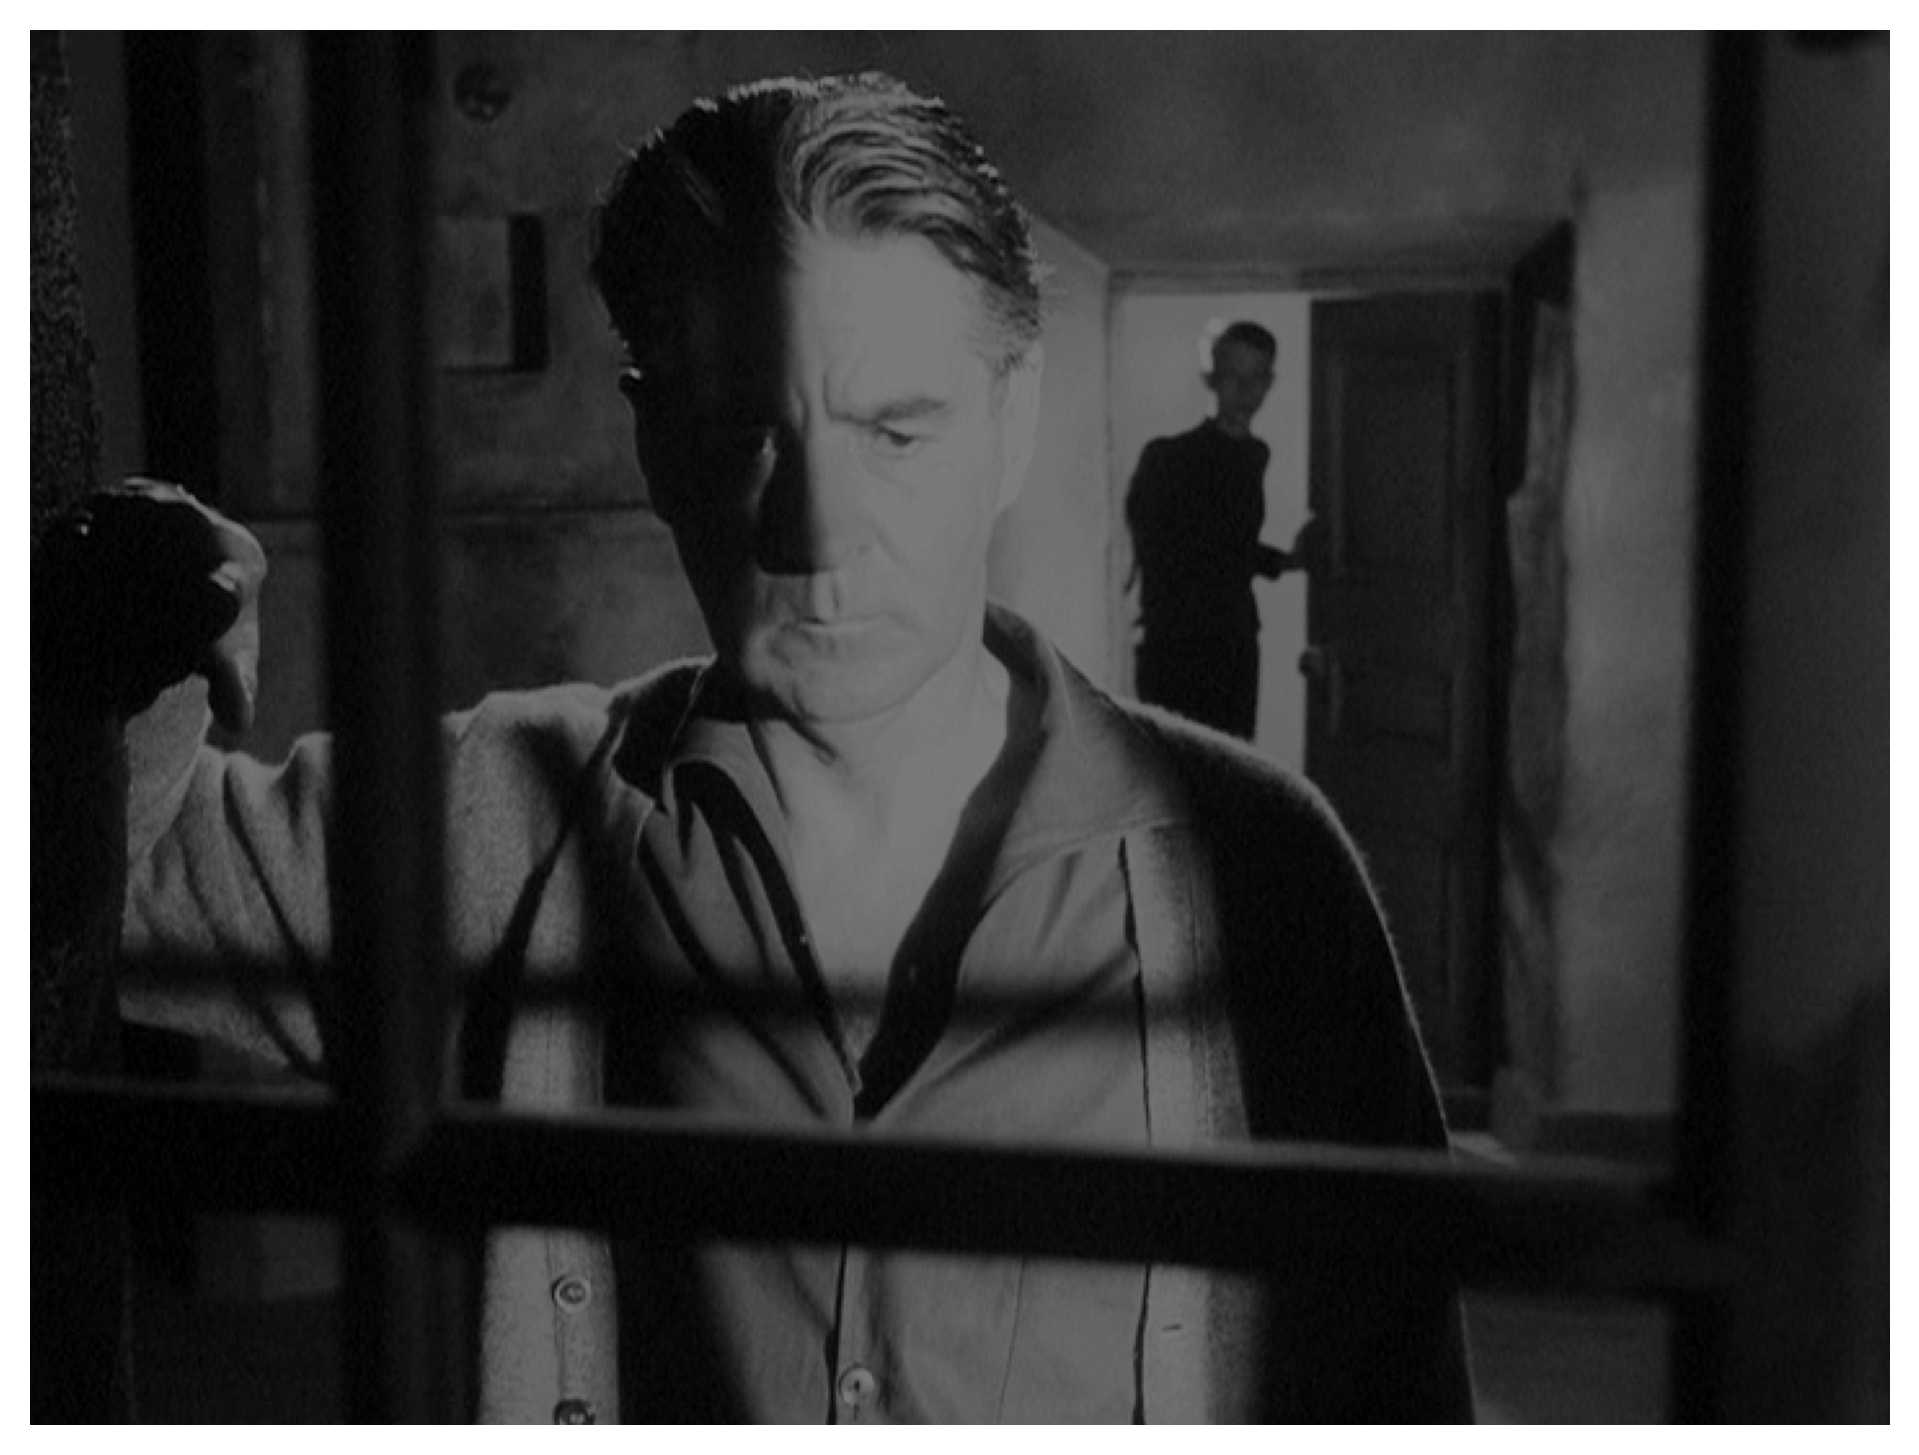
\includegraphics[width=\textwidth]{results/images/equalized_non-greedy.png}
        \caption{Non-Greedy Equalization}
    \end{subfigure}
    \hfill
    \begin{subfigure}{0.32\textwidth}
        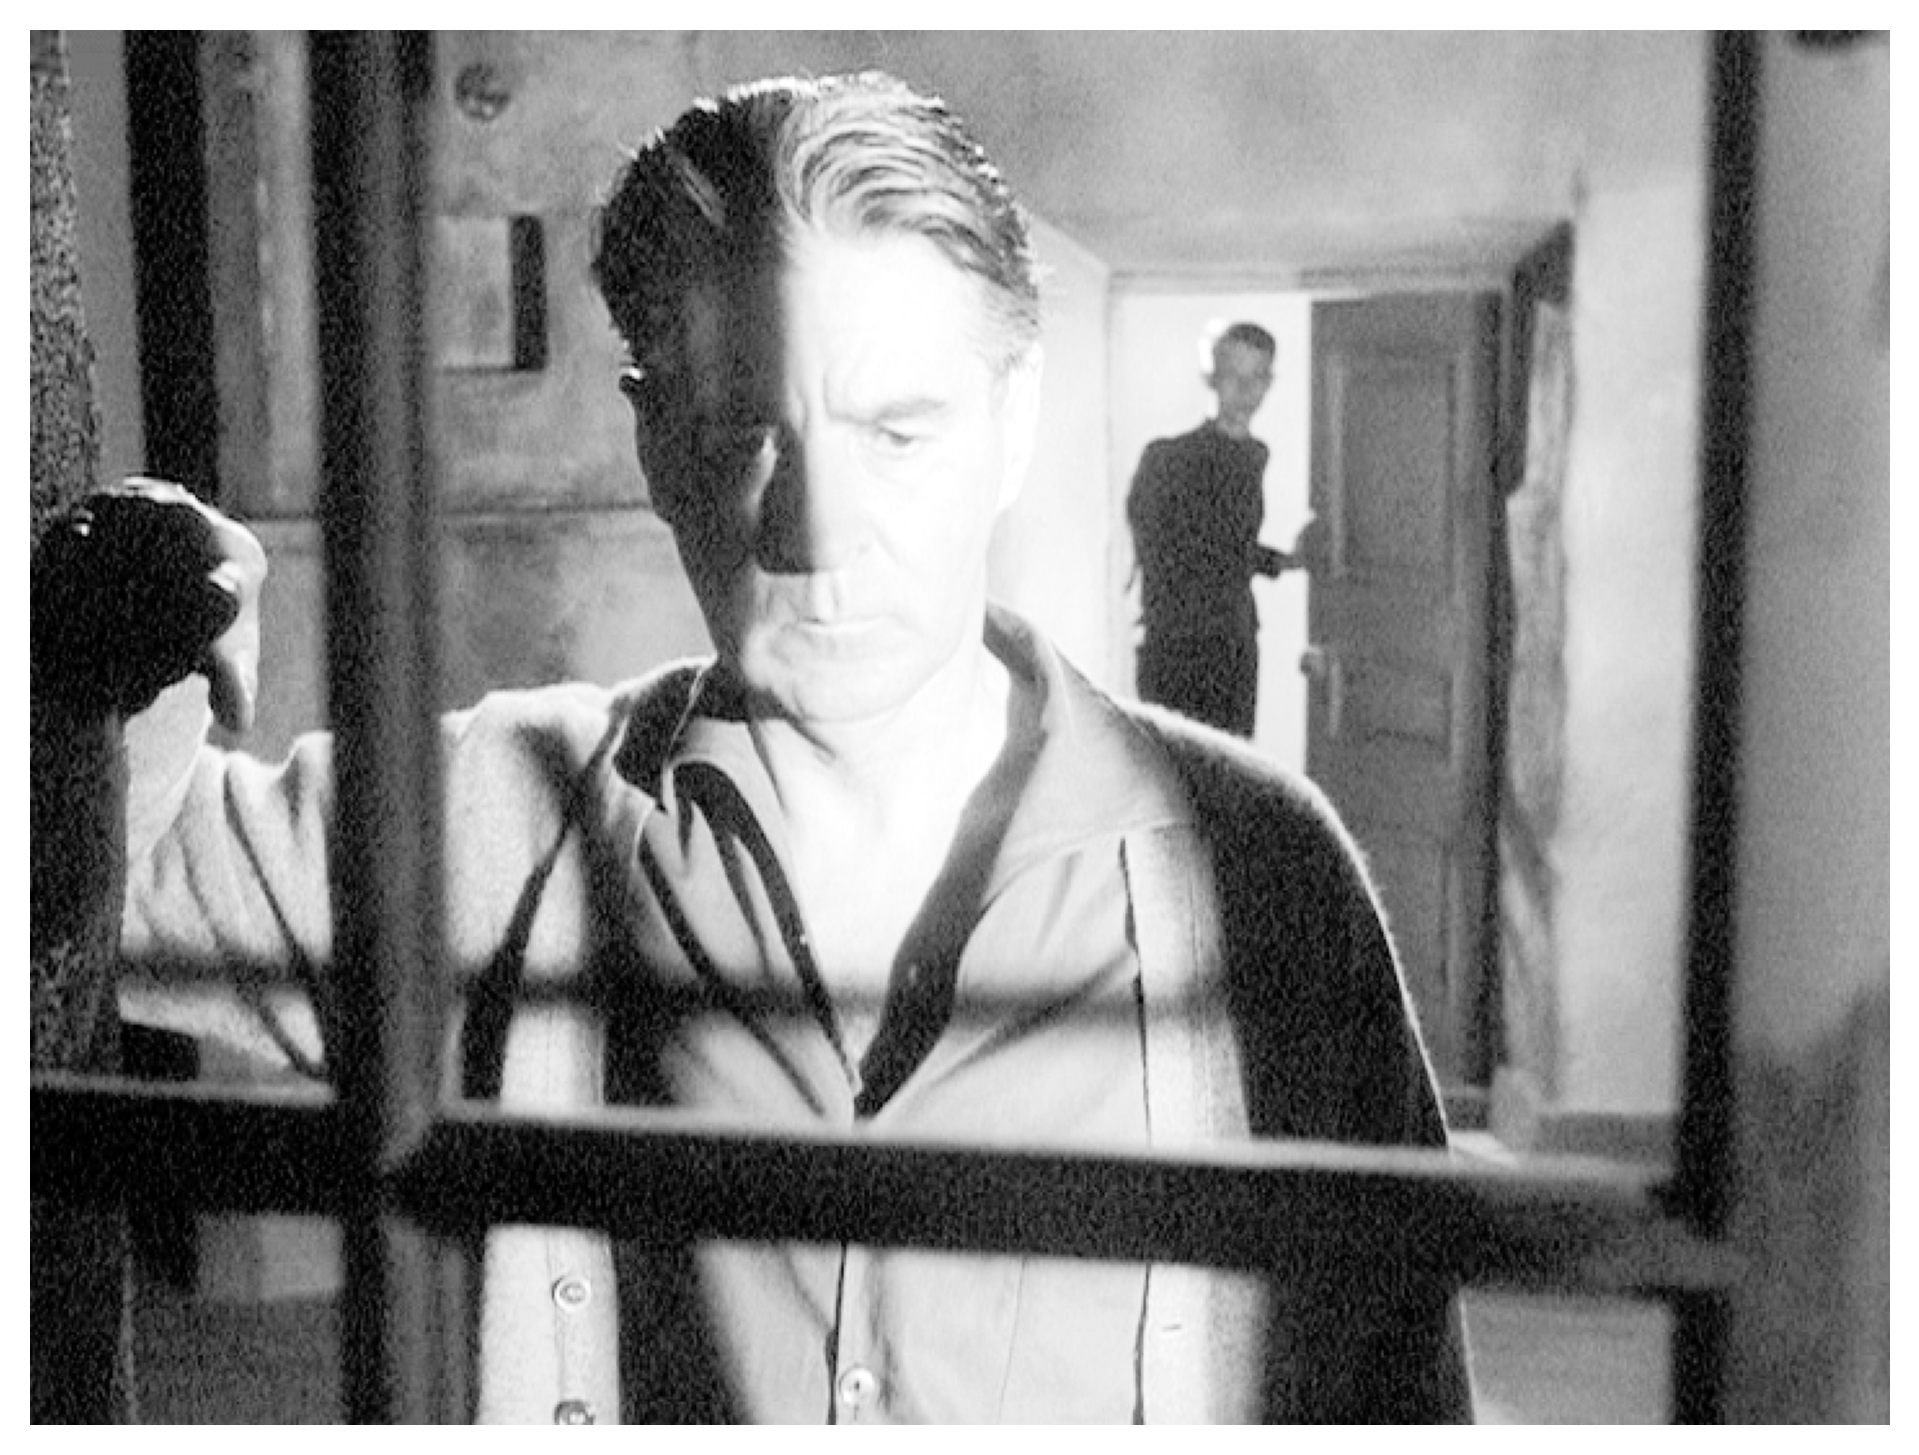
\includegraphics[width=\textwidth]{results/images/equalized_post-disturbance.png}
        \caption{Post-Disturbance Equaliz.}
    \end{subfigure}
    \caption{Side-by-side comparison of equalized images using different algorithms}
    \label{fig:eq_images}
\end{figure}


From a perceptual standpoint, each approach produce distinct visual characteristics:

\begin{itemize}
    \item \textbf{Greedy approach} produces an image with severely limited tonal range, resulting in an unnaturally dark appearance with compromised visual information. While some enhancement occurs in shadow details—such as the subtle patterns in the darker regions of the cat's body—this comes at the expense of highlight definition. The fabric texture of the couch appears flattened, and fine details in the cat's facial features are significantly obscured.
    
    \item \textbf{Non-greedy approach} also suffers from excessive darkening, though to a slightly lesser degree than the greedy method. The cat's features are more distinct, and there is better separation between the darker and lighter regions.
    
    \item \textbf{Post-disturbance approach} produces visually superior results through strategically introduced controlled noise. Shadow details in the cat's dark fur exhibit excellent micro-contrast and textural definition while simultaneously preserving subtle highlight gradations in the white chest and facial markings. Background elements demonstrate enhanced definition—particularly the vertical striping pattern of the wall, which maintains clear separation between adjacent tones. 
\end{itemize}

\subsubsection{Quantitative Performance}

Table \ref{tab:eq_metrics} presents quantitative metrics assessing how accurately each algorithm approximates the target uniform distribution. These objective measurements provide numerical validation of our visual observations, with each metric capturing different aspects of histogram similarity. The Mean Squared Error (MSE), Bhattacharyya distance, and Earth Mover's Distance (EMD) reveal divergence from the target distribution (lower values indicate better performance), while the Histogram Intersection metric measures direct overlap between distributions (higher values represent better matches). Notably, these metrics demonstrate a consistent performance ranking across all evaluation criteria.
\begin{table}[htbp]
    \centering
    \begin{tabular}{lcccc}
        \toprule
        \textbf{Algorithm} & \textbf{MSE} & \textbf{Bhattacharyya} & \textbf{EMD} & \textbf{Intersection} \\
        \midrule
        Greedy & 2.22e-05 & 0.325418 & 0.255410 & 0.554179 \\
        Non-Greedy & 1.90e-05 & 0.221164 & 0.207528 & 0.654993 \\
        Post-Disturbance & 2.34e-11 & 1.94e-07 & 0.000039 & 0.999923 \\
        \bottomrule
    \end{tabular}
    \caption{Quantitative comparison of histogram equalization algorithms}
    \label{tab:eq_metrics}
\end{table} 

% The metrics reveal dramatic differences in histogram accuracy:


\begin{itemize}
    \item \textbf{Greedy approach} shows substantial deviation from the uniform target with the highest EMD and Bhattacharyya distance of all methods. With only 55.4\% histogram intersection, it fails to effectively approximate the target uniform distribution.
    
    \item \textbf{Non-greedy approach} performs moderately better than the greedy method, with approximately 14\% lower MSE (1.90e-05 vs. 2.22e-05) and improved histogram intersection (65.5\% vs. 55.4\%). While this represents a meaningful improvement, the algorithm still produces significant deviations from the ideal uniform distribution.
    
    \item \textbf{Post-disturbance approach} demonstrates extraordinary accuracy, with MSE approximately six orders of magnitude lower than the other methods. Its EMD value is over 5,000 times smaller than the greedy approach, and its histogram intersection score approaches the theoretical maximum of 1.0, indicating nearly perfect uniformity.
\end{itemize}
\subsection{Histogram Matching}

\subsubsection{Visual Results}

Figure~\ref{fig:match_comp} illustrates the performance of the three histogram matching algorithms. The left column shows the reference image and the results of applying each matching method to the input image. The right column displays the corresponding histograms, with the target reference histogram overlaid as a purple line for direct comparison.

\begin{figure}[H]
    \centering
    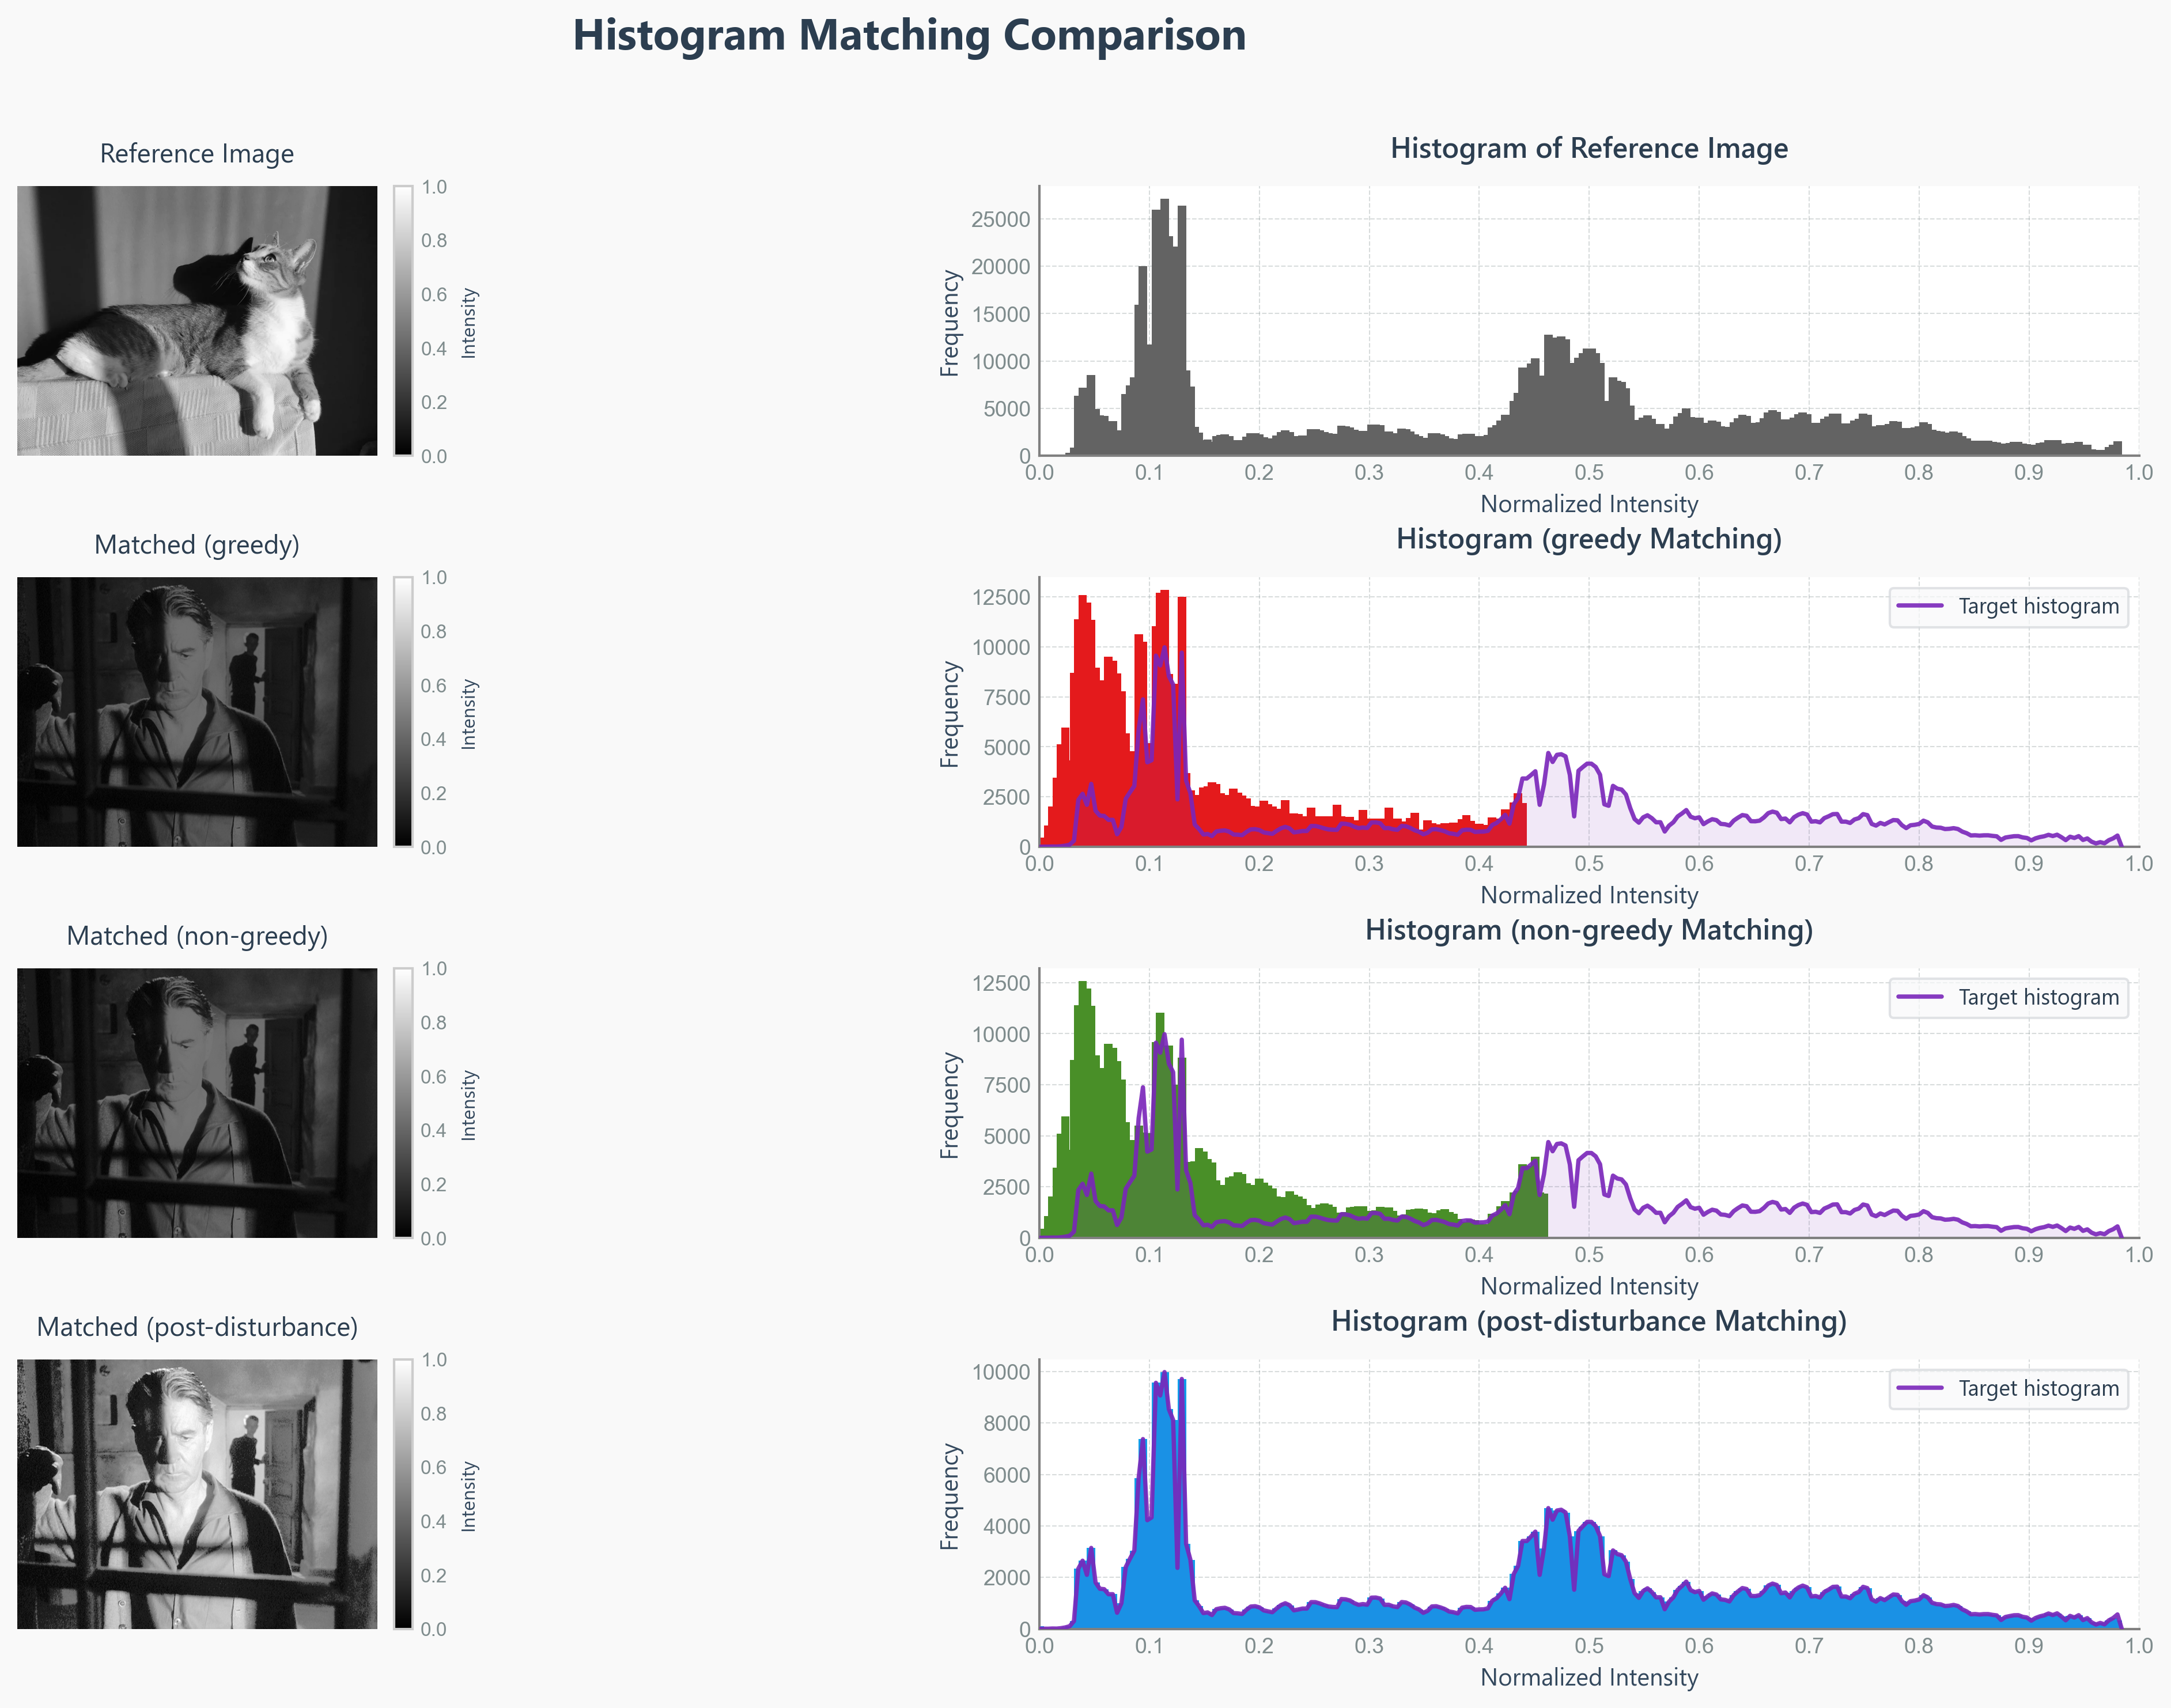
\includegraphics[width=\textwidth]{results/images/histogram_matching_comparison.png}
    \caption{Comparison of Histogram Matching Modes.}
    \label{fig:match_comp}
\end{figure}


\subsubsection{Histogram Analysis}

The matched histograms reveal algorithm-specific characteristics when attempting to reproduce the reference distribution:

\begin{itemize}
    \item \textbf{Reference Histogram:} The target distribution (purple line) reflects a grayscale portrait with significant concentration in the dark tones (0.0-0.1), gradual tapering toward the mid-tones (0.1-0.3), and limited presence in the highlight regions (beyond 0.4) with nearly no pixels in the brightest areas (0.7-1.0). This characteristic distribution represents a low-key, high-contrast image typical of film noir or dramatic portrait photography, with strong shadows and limited highlight detail.
    
    \item \textbf{Greedy Matching:} The resulting histogram attempts to follow the general shape of the reference but deviates significantly with pronounced, isolated peaks. Particularly notable are extreme peaks in the shadow regions (0.0-0.15) that greatly exceed the target frequency. The overall envelope roughly follows the target histogram's decay pattern, but with pronounced local irregularities throughout the intensity range. 
     
    \item \textbf{Non-Greedy Matching:} This histogram aligns more closely with the reference curve, showing better alignment with the target curve's shape across most of the range. Excellent tracking of the reference curve occurs until approximately the 0.6 intensity value. A notable deviation occurs beyond this intensity value, where the matched histogram shows virtually no pixels despite the reference having a small but visible presence in the 0.6-0.7 range.
    
    \item \textbf{Post-Disturbance Matching:} This histogram demonstrates remarkable fidelity to the reference distribution, with the green output curve virtually indistinguishable from the purple target line. The noise-based approach successfully breaks up discrete input intensity groups, enabling precise mapping to the target distribution across the entire intensity range.
\end{itemize}

\subsubsection{Visual Quality Assessment}

Figure~\ref{fig:match_images} provides a side-by-side comparison of the three matched images for detailed examination.

\begin{figure}[H]
    \centering
    \begin{subfigure}{0.32\textwidth}
        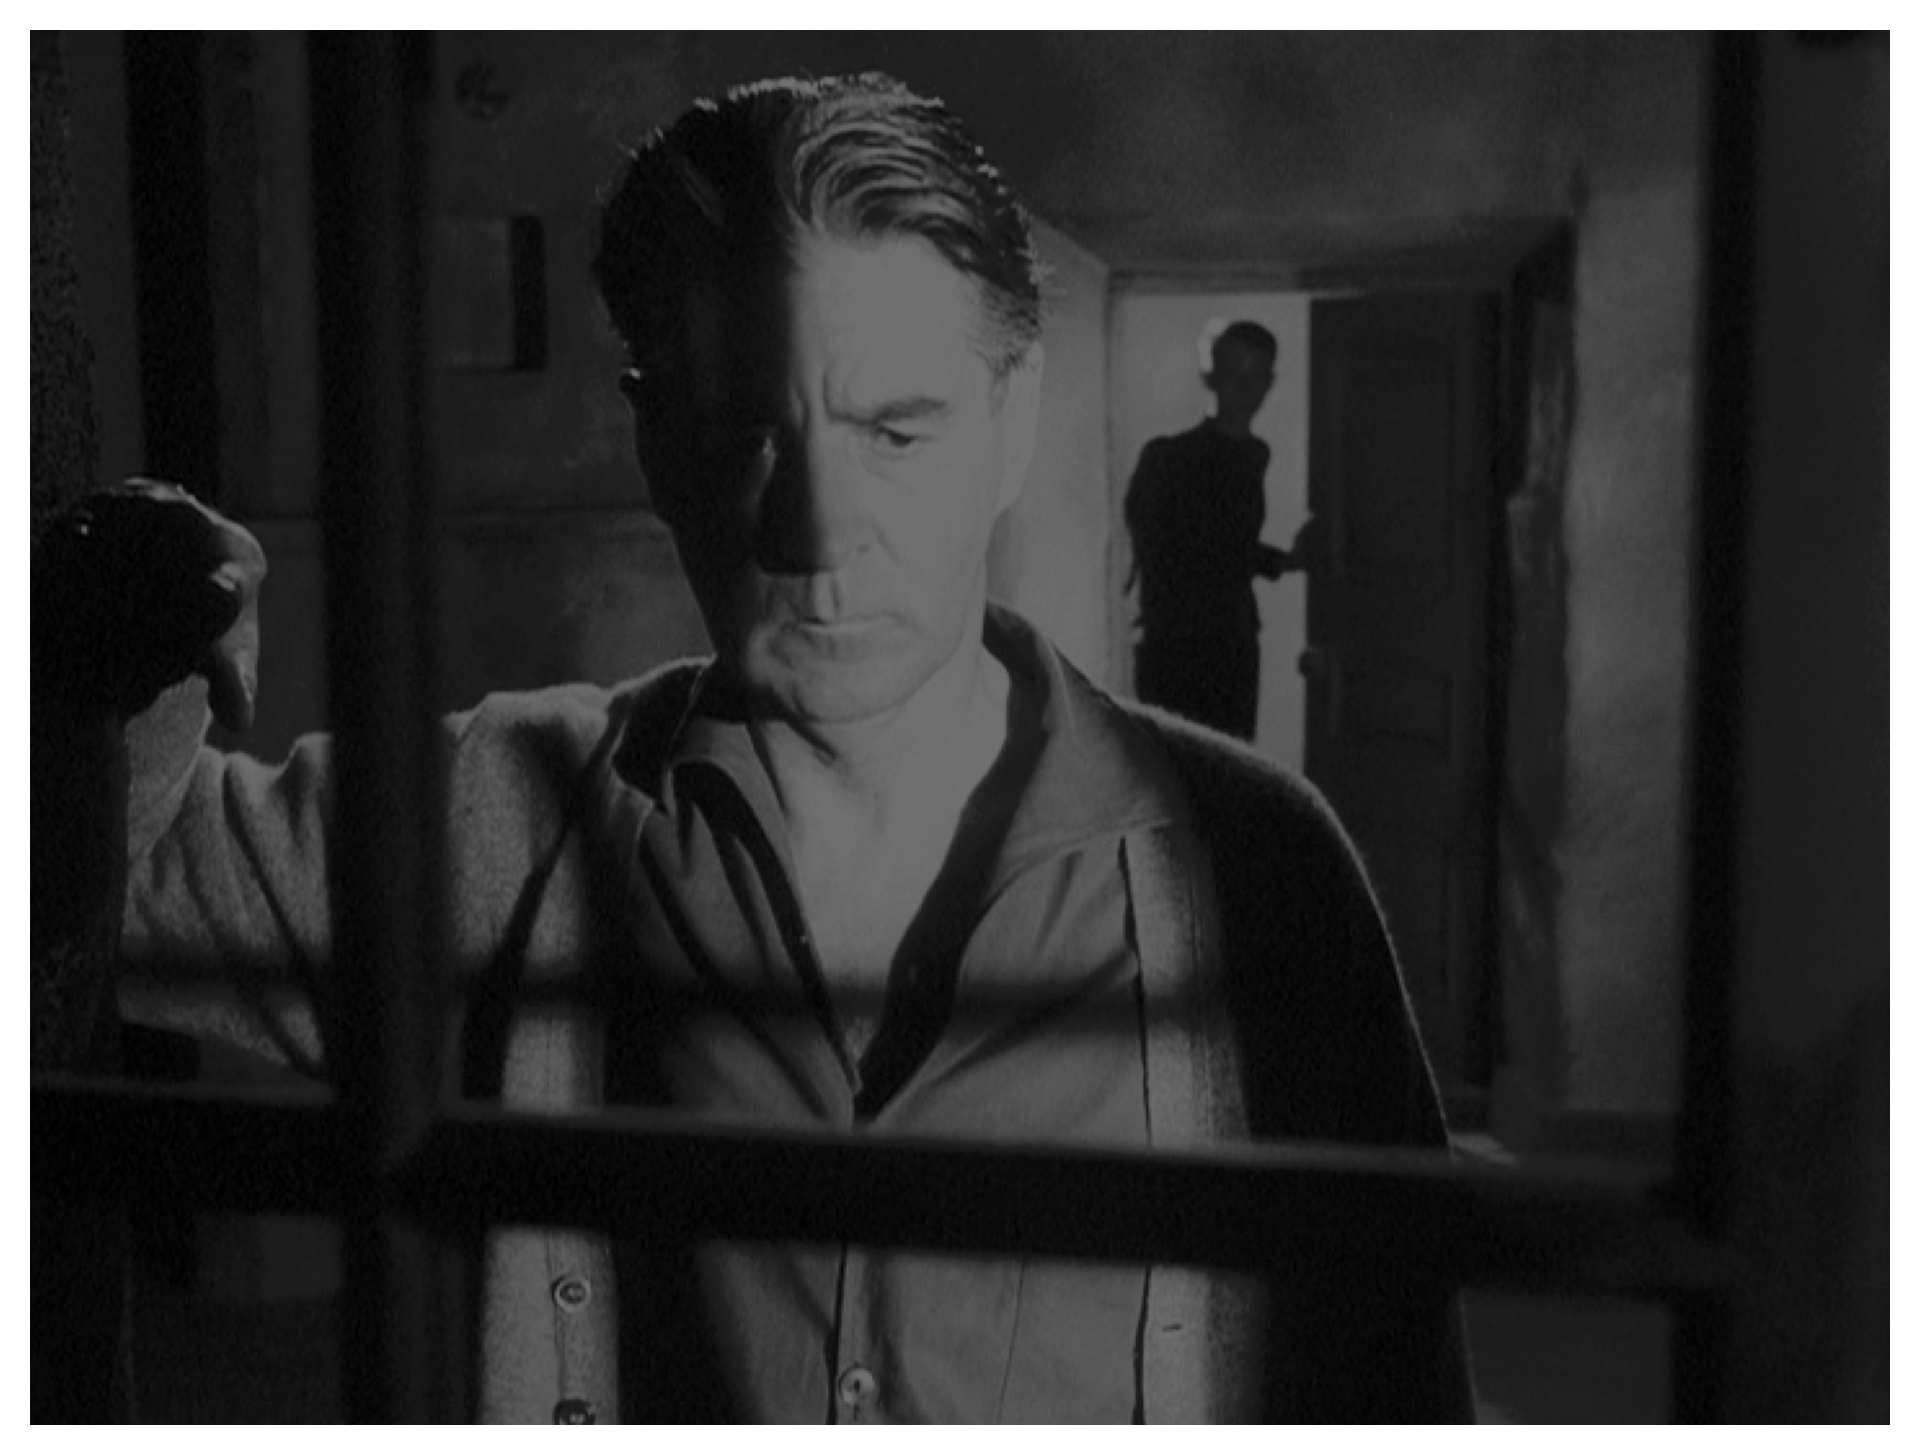
\includegraphics[width=\textwidth]{results/images/matched_greedy.png}
        \caption{Greedy Matching}
    \end{subfigure}
    \hfill
    \begin{subfigure}{0.32\textwidth}
        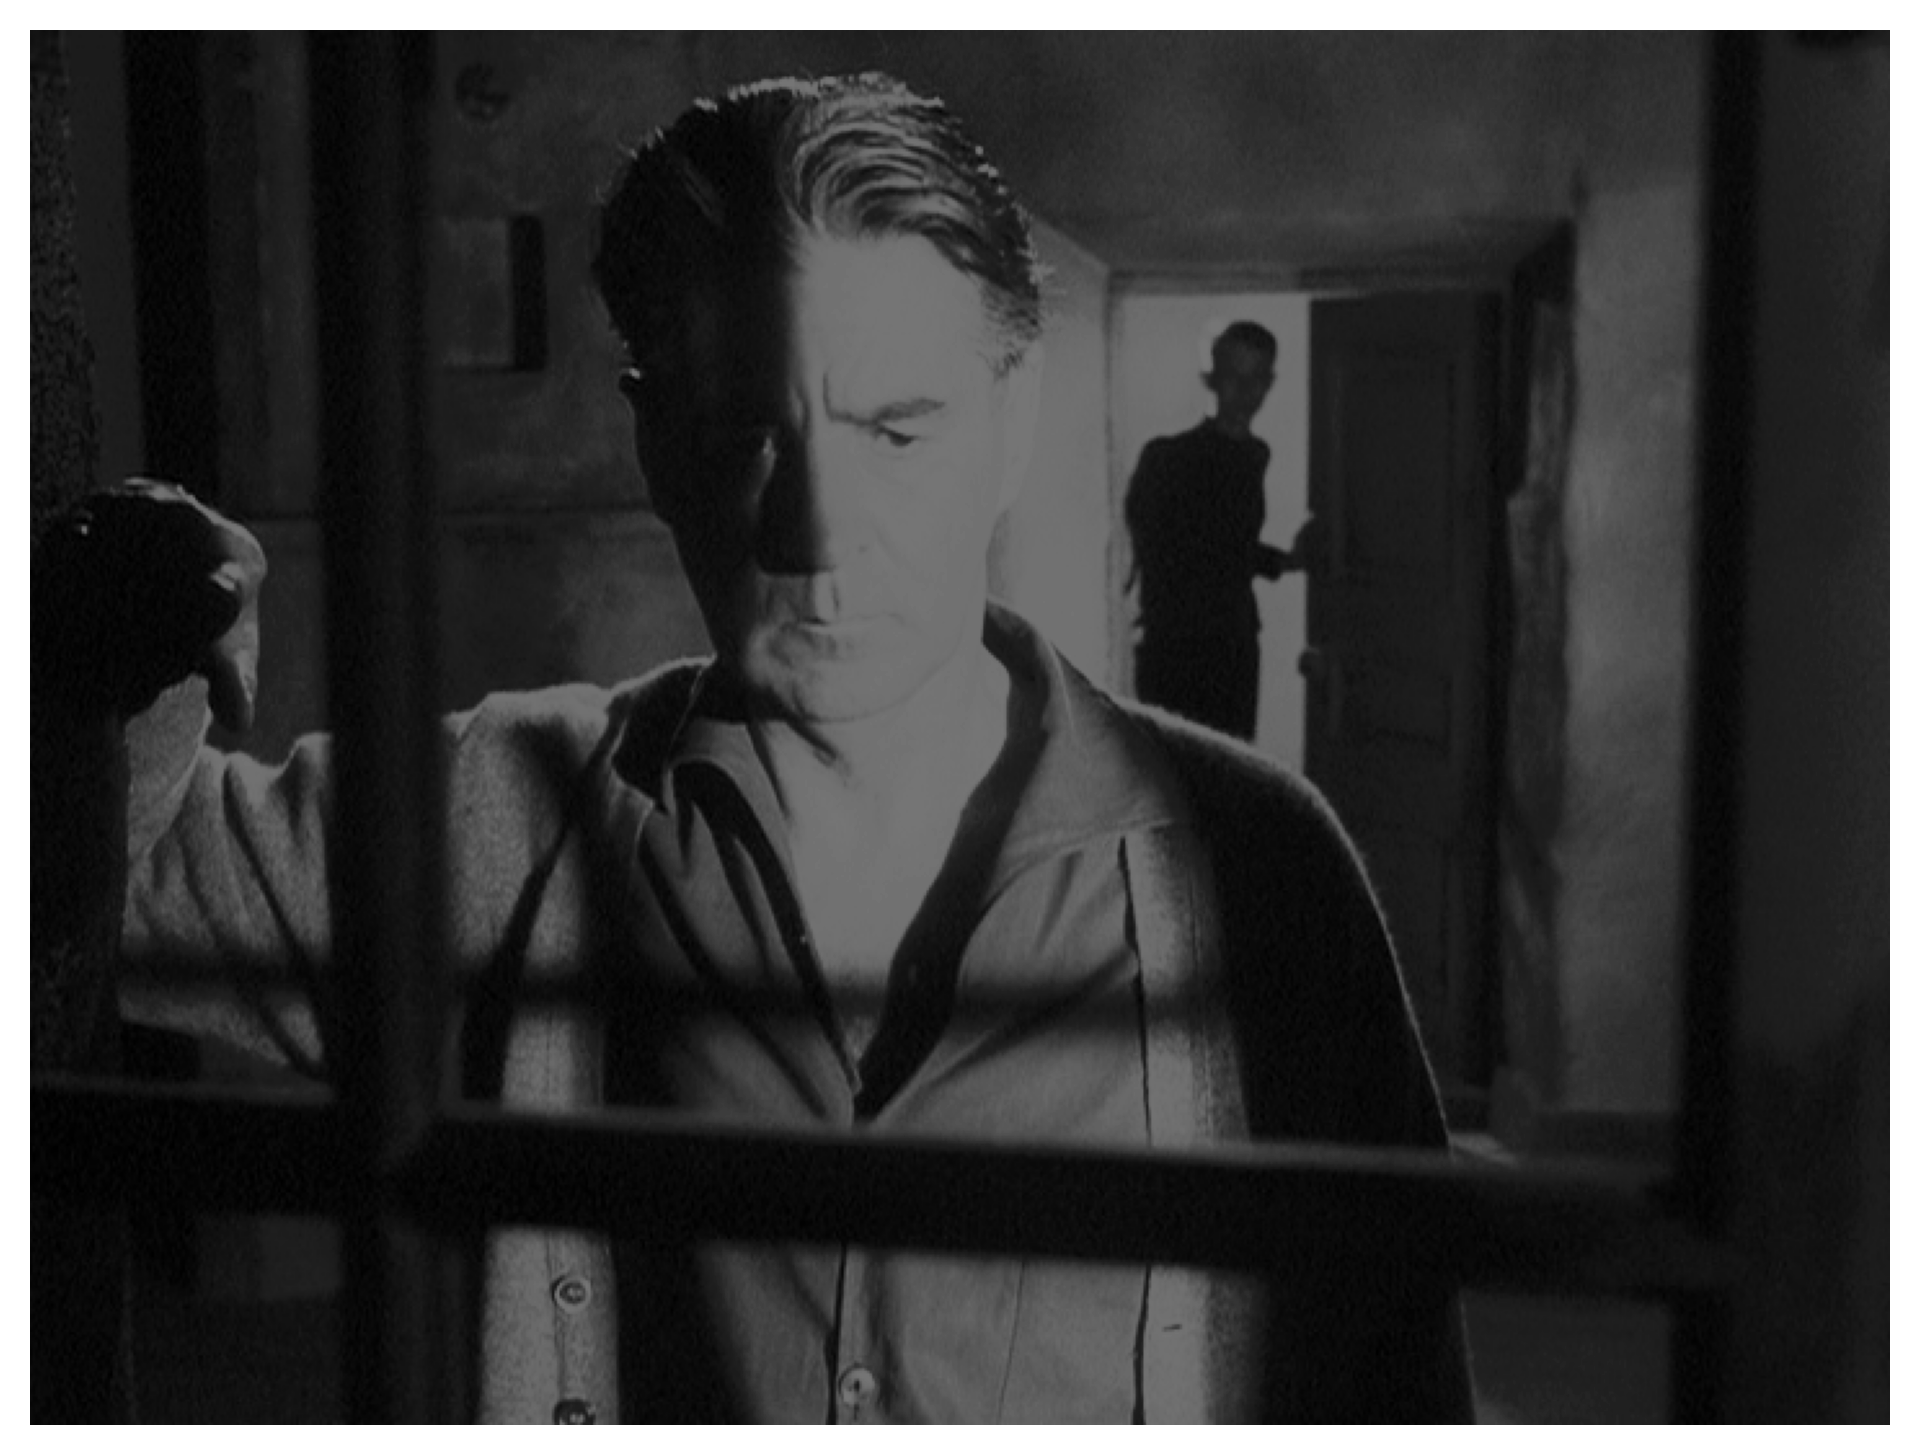
\includegraphics[width=\textwidth]{results/images/matched_non-greedy.png}
        \caption{Non-Greedy Matching}
    \end{subfigure}
    \hfill
    \begin{subfigure}{0.32\textwidth}
        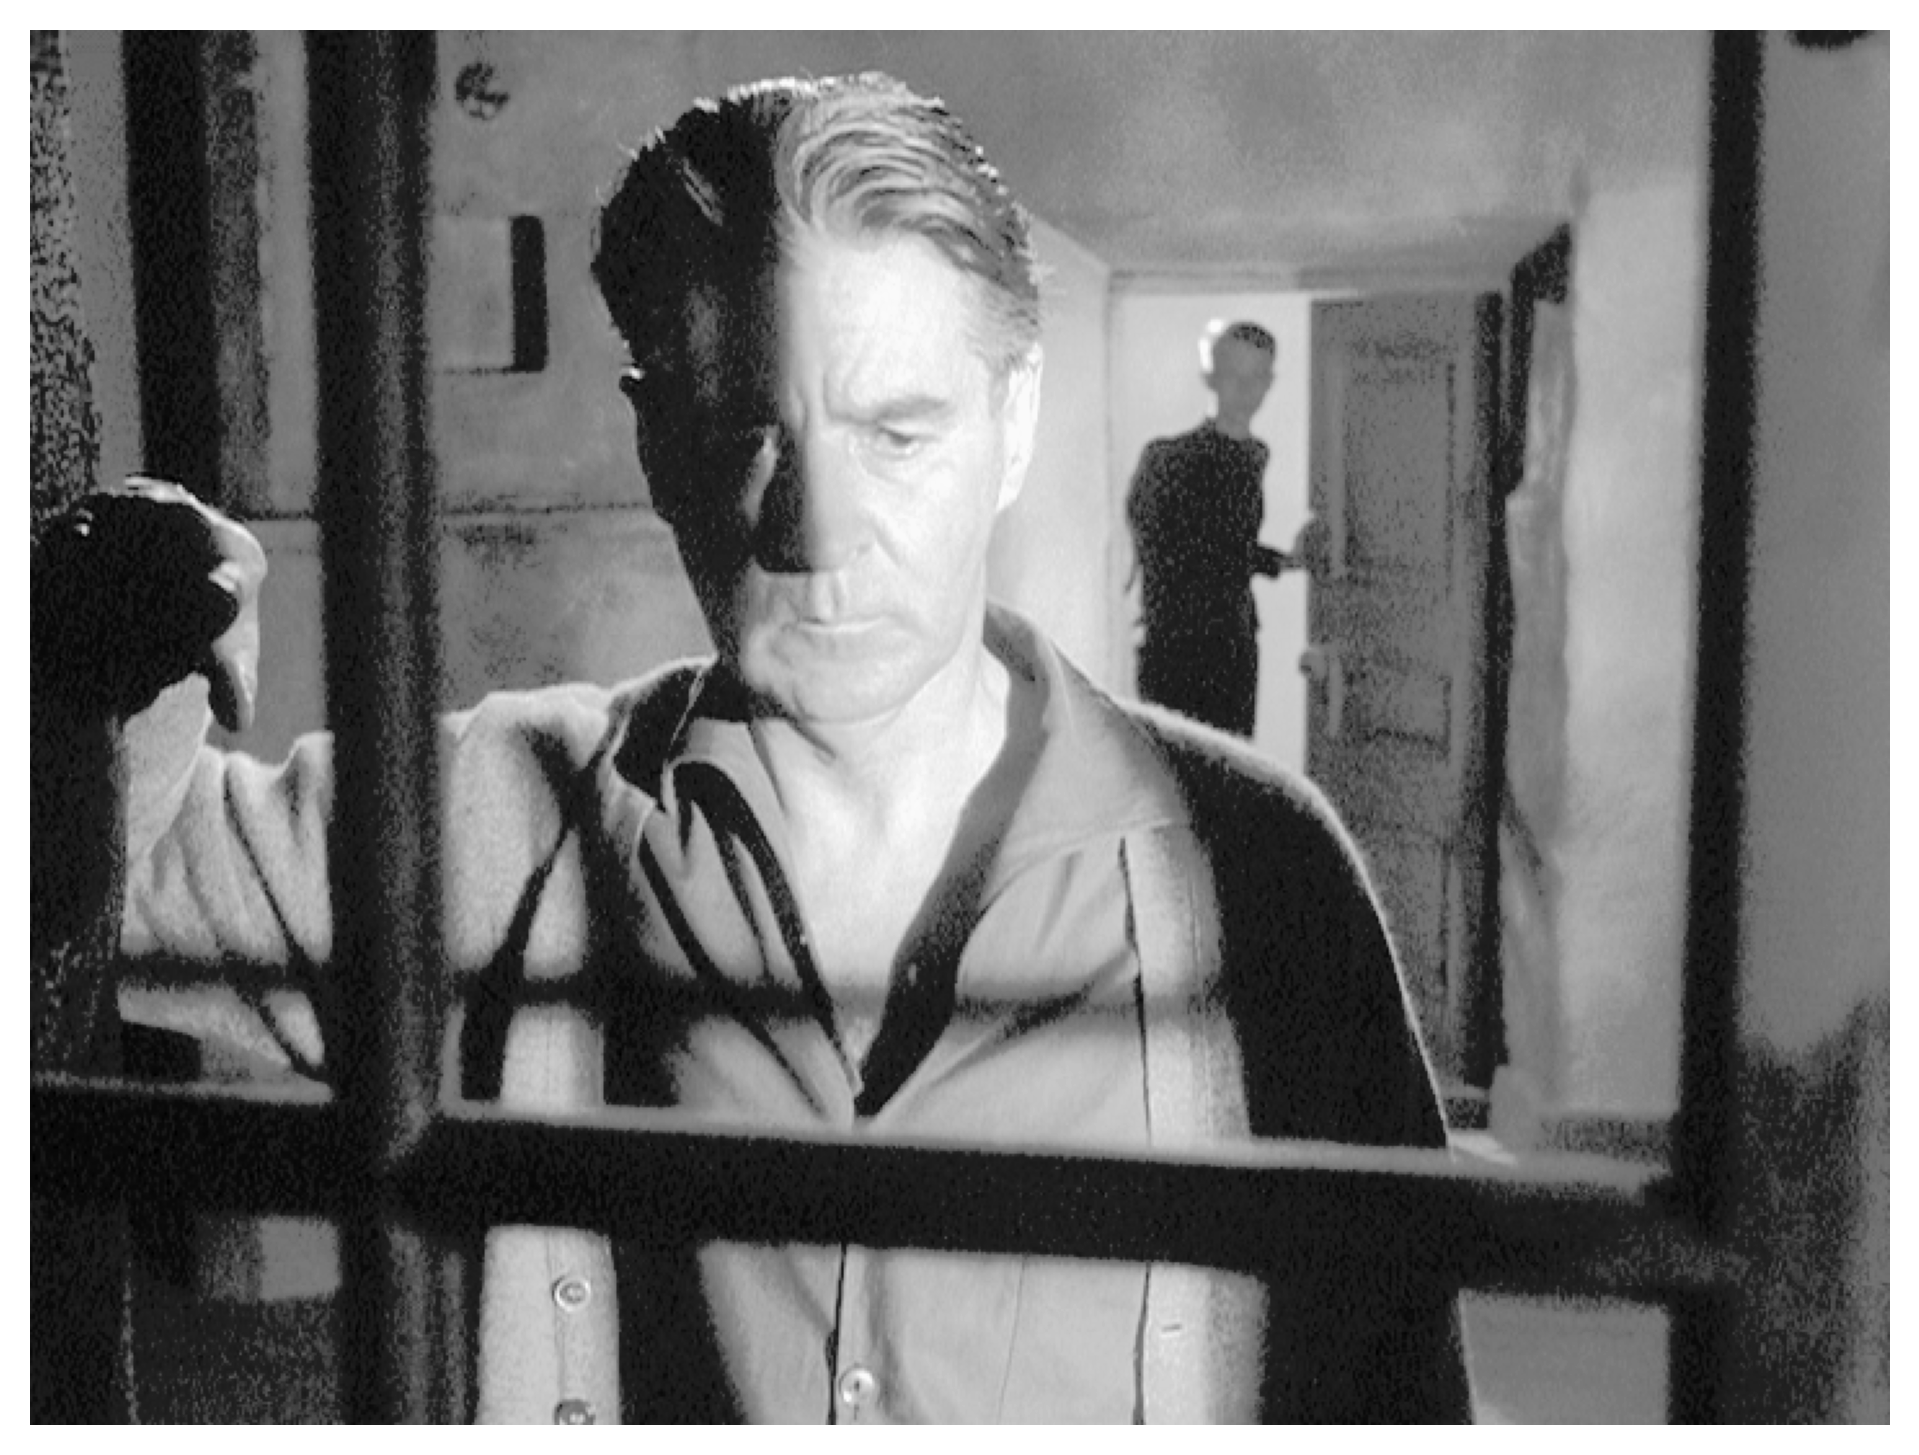
\includegraphics[width=\textwidth]{results/images/matched_post-disturbance.png}
        \caption{Post-Disturbance Match.}
    \end{subfigure}
    \caption{Comparison of histogram-matched images using different algorithms}
    \label{fig:match_images}
\end{figure}



Each matching algorithm creates distinctive visual characteristics while attempting to transfer the tonal properties of the reference image:

\begin{itemize}
    \item \textbf{Greedy approach} transforms the input image into an excessively dark result that severely compromises visibility of important details. The image appears unnaturally compressed into the lowest intensity range, creating a muddy, indistinct representation where the cat's features become difficult to discern. This aggressive darkness fails to preserve the subtle tonal variations present in the original image while attempting to match the reference image's.

    
    \item \textbf{Non-greedy approach} yields a more balanced result that better preserves the original image's details while effectively adopting the reference image's tonal characteristics. Though still predominantly dark, this version maintains distinguishable textures and features throughout. The cat's facial details remain visible, with discernible separation between light and dark fur patterns. The texture of the couch fabric can still be identified, and mid-tone details maintain better definition than in the greedy version. The overall image achieves a dramatic low-key aesthetic similar to the reference while retaining meaningful visual information.
    
    \item \textbf{Post-disturbance approach} achieves superior visual quality, successfully transferring the reference image's film noir-like tonal properties while preserving intricate details in the original image. The cat's facial features, particularly the eyes and whiskers, remain crisp and well-defined despite the significant darkening effect. The white chest fur maintains subtle gradations of brightness rather than collapsing into uniform gray areas. Background elements show clear separation with visible textures in the wall and couch. The overall image exhibits smooth, natural transitions between intensity levels, creating a result that faithfully captures the dramatic lighting character of the reference image without sacrificing the original detail.
\end{itemize}

\subsubsection{Quantitative Performance}

Table \ref{tab:match_metrics} quantifies how accurately each algorithm reproduces the reference histogram, providing objective measures that validate the visual observations.

\begin{table}[htbp]
    \centering
    \begin{tabular}{lcccc}
        \toprule
        \textbf{Algorithm} & \textbf{MSE} & \textbf{Bhattacharyya} & \textbf{EMD} & \textbf{Intersection} \\
        \midrule
        Greedy & 9.05e-06 & 0.127502 & 0.070187 & 0.782954 \\
        Non-Greedy & 2.75e-06 & 0.020500 & 0.009070 & 0.897568 \\
        Post-Disturbance & 3.99e-12 & 0.000047 & 0.000044 & 0.999899 \\
        \bottomrule
    \end{tabular}
    \caption{Quantitative comparison of histogram matching algorithms.}
    \label{tab:match_metrics}
\end{table}

The metrics reveal a clear performance hierarchy across all measures:
\begin{itemize}
    \item \textbf{Greedy approach} shows significant deviation from the reference histogram with the highest EMD and Bhattacharyya distance among all methods. With a 78.3\% histogram intersection value, it provides a reasonable approximation of the target distribution's general shape but fails to accurately capture its precise characteristics, particularly in handling the pronounced peaks in shadow regions.
    
    \item \textbf{Non-greedy approach} performs substantially better than the greedy method, with approximately 70\% lower MSE (2.75e-06 vs. 9.05e-06) and improved histogram intersection (89.8\% vs. 78.3\%). The Bhattacharyya distance is approximately six times lower and EMD almost eight times lower, indicating much more accurate distribution matching while still maintaining computational efficiency.
    
    \item \textbf{Post-disturbance approach} demonstrates exceptional accuracy, with MSE approximately six orders of magnitude lower than the greedy method and three orders of magnitude lower than the non-greedy approach, while its histogram intersection almost perfectly matches the theoretical maximum of 1.0, indicating nearly exact reproduction of the reference distribution.
\end{itemize}



\newpage


\appendix

\section{Post-Processing Stretching for Dynamic Range Enhancement}\label{appendix:stretching}

\subsection{Addressing the Limited Dynamic Range Problem}

As identified in Section~\ref{HistogramAnalysis}, a key limitation of both the greedy and non-greedy approaches is their failure to utilize the full dynamic range. This occurs because large input intensity groups are assigned to single output bins, causing early bin saturation. Consequently, higher-intensity output bins remain empty, particularly in the upper end of the histogram (0.6-1.0 range), which results in visibly darker output images.

To overcome this limitation, we can apply a simple post-processing stretching operation, commonly known as contrast stretching or normalization. The process works by linearly rescaling the histogram-equalized image to span the full [0,1] range:

\begin{equation}
I_{stretched}(x,y) = \frac{I_{equalized}(x,y) - I_{min}}{I_{max} - I_{min}}
\end{equation}

where $I_{min}$ and $I_{max}$ are the min and max intensity values in the equalized image.

\subsection{Experimental Results with Stretching}

Figure \ref{fig:stretch_comp} presents a comparison of the greedy and non-greedy equalization results before and after applying the stretching operation.

\begin{figure}[H]
    \centering
    \includegraphics[width=\textwidth]{results/images/histogram_equalization_with_stretch.png}
    \caption{Comparison of Histogram Equalization Modes after applying stretching}
    \label{fig:stretch_comp}
\end{figure}

\subsubsection{Visual Quality Assessment}

\begin{figure}[H]
    \centering
    \begin{subfigure}{0.48\textwidth}
        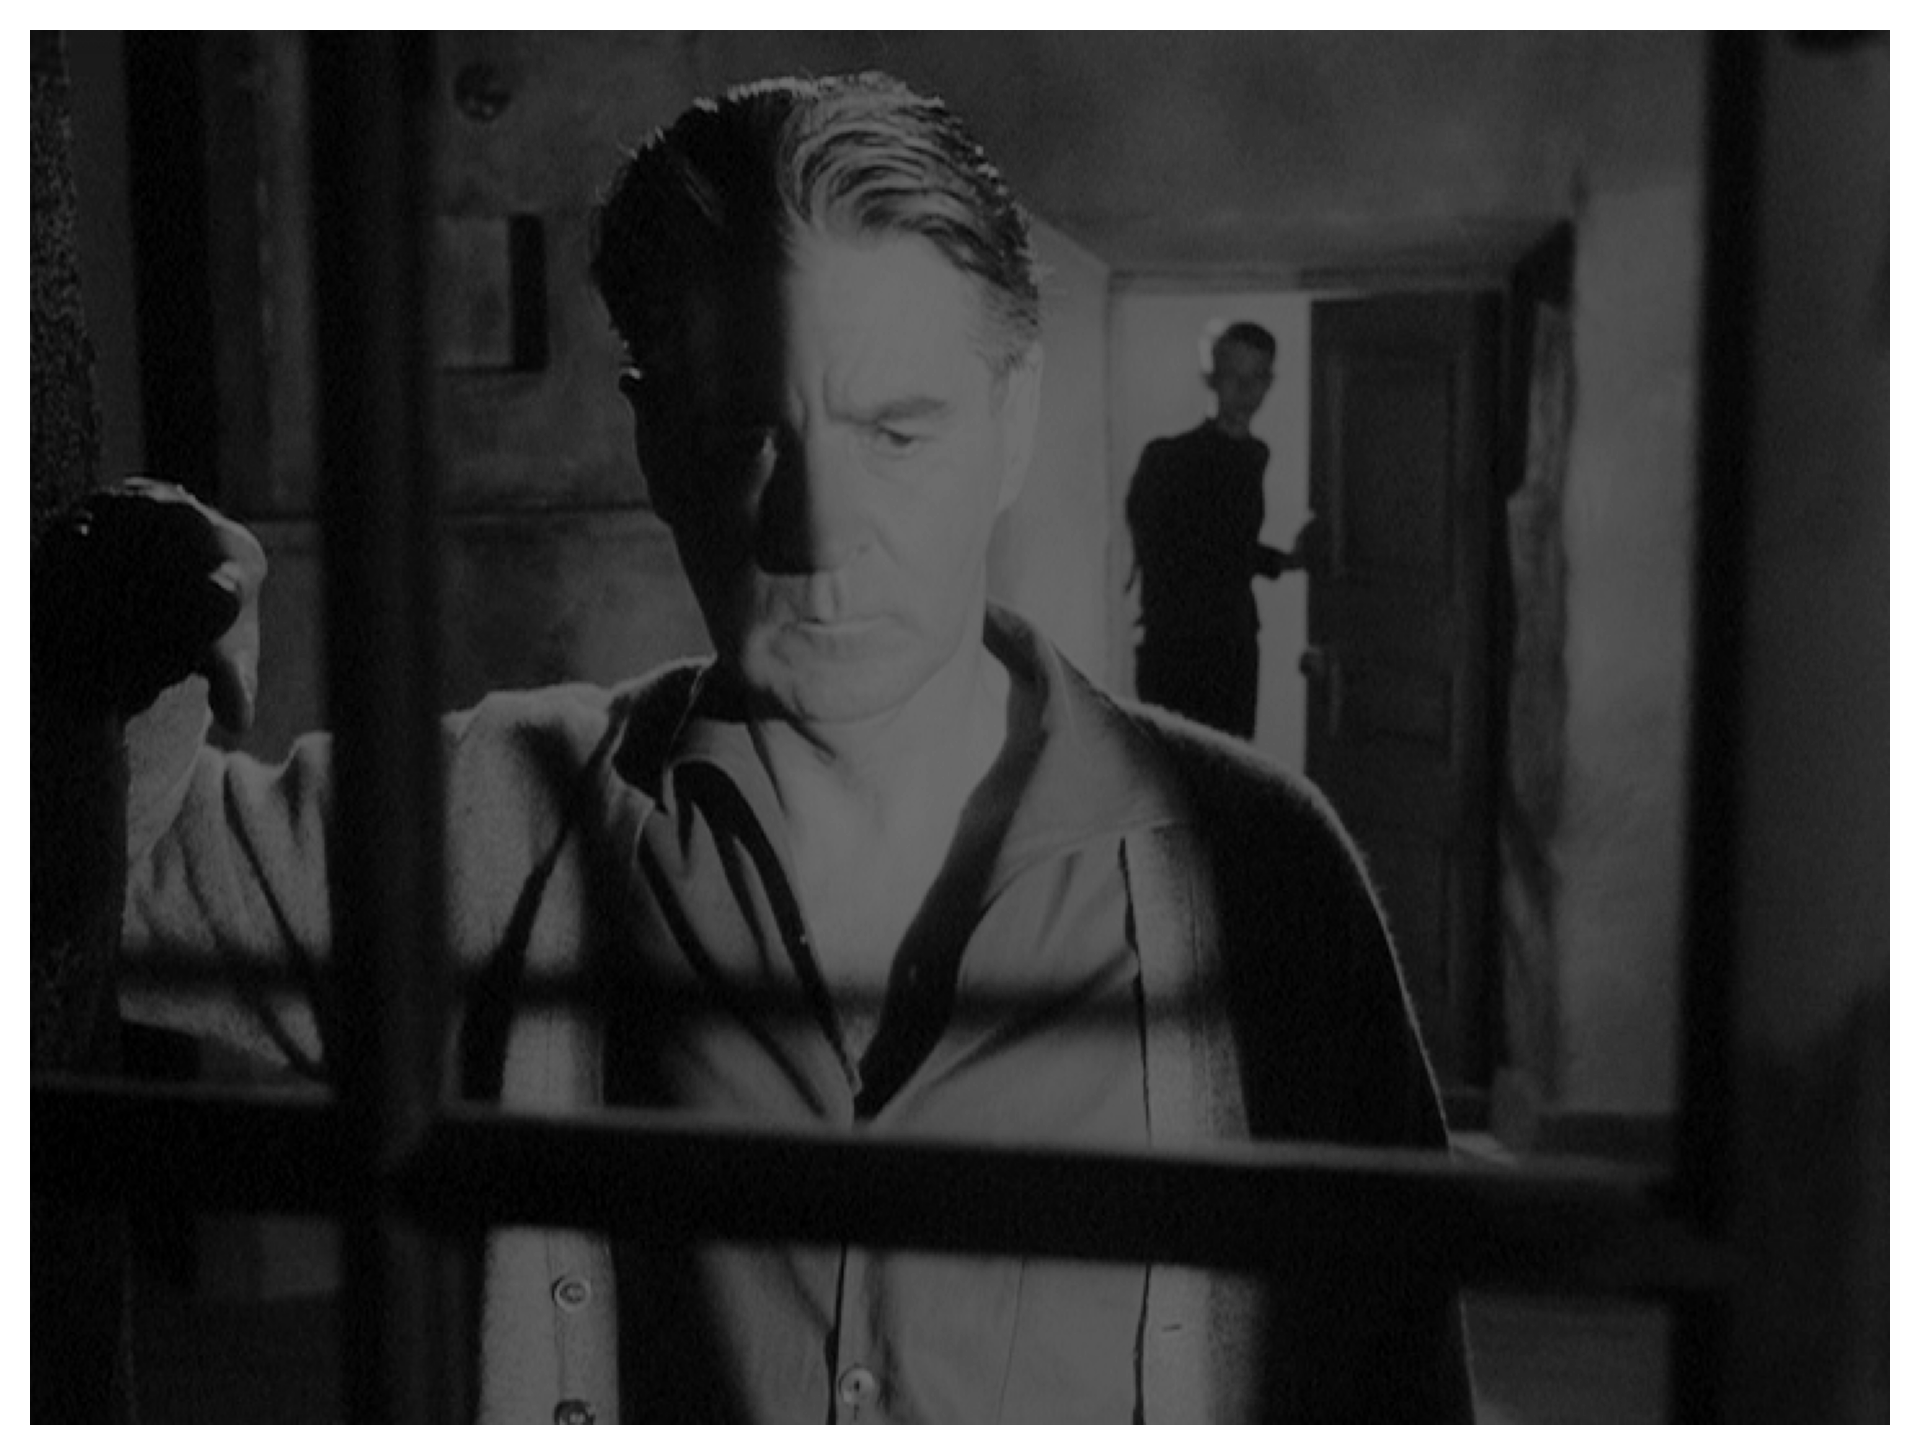
\includegraphics[width=\textwidth]{results/images/equalized_greedy.png}
        \caption{Greedy}
    \end{subfigure}
    \hfill
    \begin{subfigure}{0.48\textwidth}
        \includegraphics[width=\textwidth]{results/images/equalized_greedy_stretched.png}
        \caption{Greedy + Stretch}
    \end{subfigure}
    
    \vspace{0.5cm}
    
    \begin{subfigure}{0.48\textwidth}
        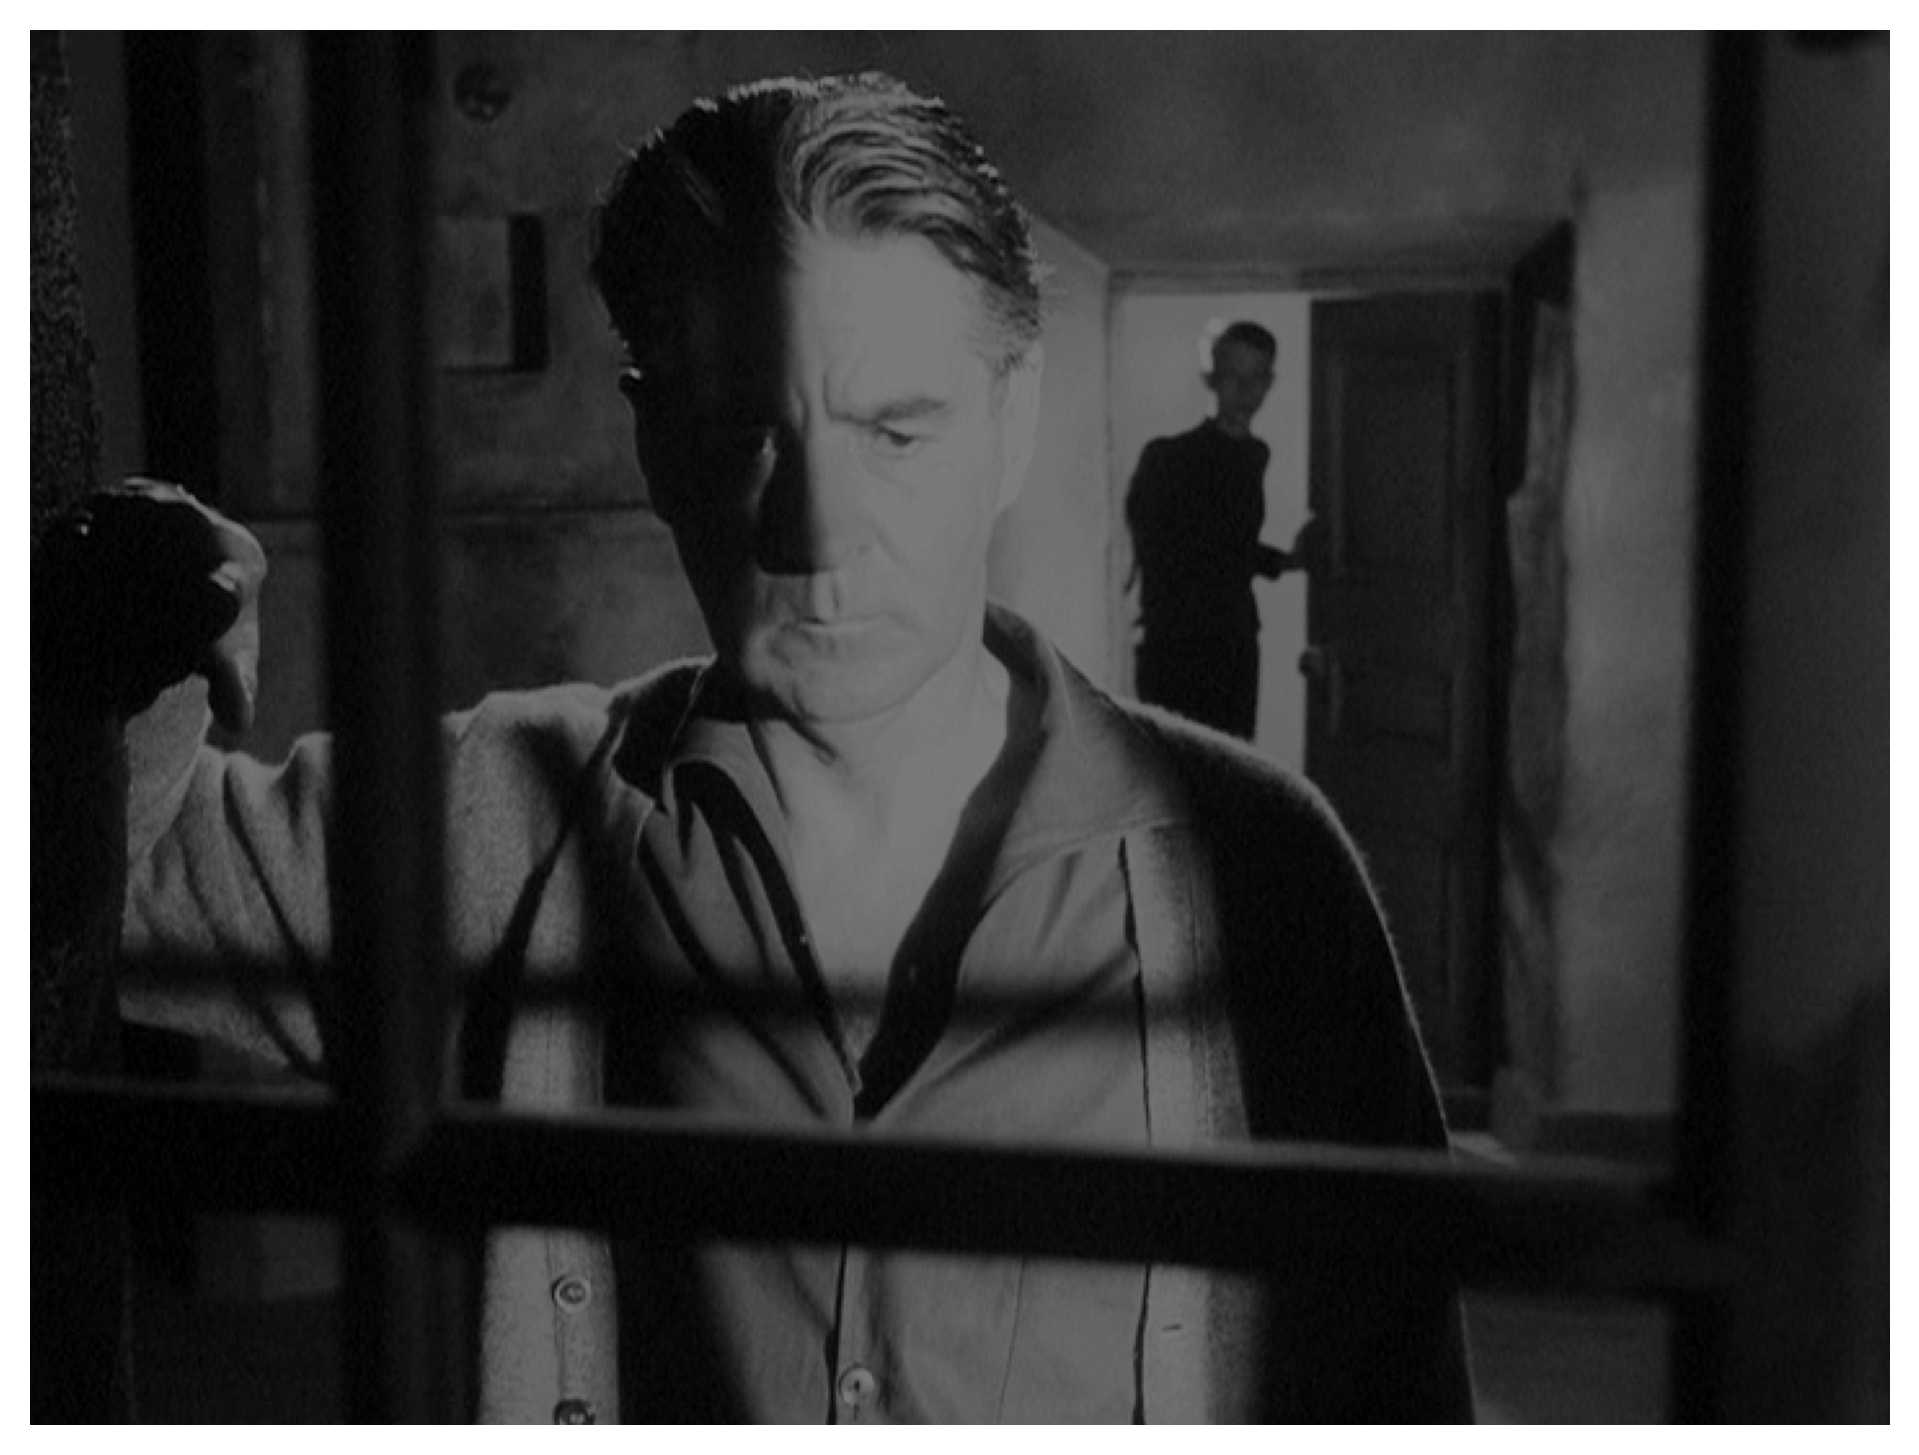
\includegraphics[width=\textwidth]{results/images/equalized_non-greedy.png}
        \caption{Non-Greedy}
    \end{subfigure}
    \hfill
    \begin{subfigure}{0.48\textwidth}
        \includegraphics[width=\textwidth]{results/images/equalized_non-greedy_stretched.png}
        \caption{Non-Greedy + Stretch}
    \end{subfigure}
    \caption{Visual comparison of histogram equalization before and after applying stretching}
    \label{fig:stretch_comparison}
\end{figure}

The visual impact of stretching is immediately apparent:

\begin{itemize}
    \item \textbf{Greedy Approach:} The stretched version shows dramatically improved brightness and contrast compared to the original equalized image. Details in the mid-tone and highlight regions that were previously compressed into a narrow intensity range are now fully revealed. The cat's facial features become remarkably more defined, with the white/light areas of the fur displaying significantly enhanced detail and texture. The couch fabric pattern, barely discernible in the original equalized version, now shows clear textural definition. 
    
    \item \textbf{Non-Greedy Approach:} While the improvement is less dramatic than for the greedy method, stretching still provides substantial enhancement to the overall contrast. The image appears more visually balanced with finer separation between tonal regions, particularly in highlight areas that were previously underutilized. The white areas of the cat's fur gain additional definition, and subtle gradations in the cat's face and body become more apparent.
\end{itemize}







\end{document}